%%%%%%%%%%%%%%%%%%%%%%%%%%%%%%%%%%%%%%%%%12pt: grandezza carattere
                                        %a4paper: formato a4
                                        %openright: apre i capitoli a destra
                                        %twoside: serve per fare un
                                        %   documento fronteretro
                                        %report: stile tesi (oppure book)
\documentclass[12pt,a4paper,openright,twoside]{report}
%\usepackage[english]{babel}
\usepackage[english]{babel}
\usepackage[latin1]{inputenc}
\usepackage{fancyhdr}
\usepackage{indentfirst}
\usepackage{graphicx}
\usepackage{newlfont}
\usepackage{amssymb}
\usepackage{amsmath}
\usepackage{latexsym}
\usepackage{amsthm}
\usepackage{hyperref}
\usepackage{listings}
\usepackage[table,xcdraw]{xcolor}
\usepackage{multirow}
\usepackage[bottom]{footmisc}

\oddsidemargin=30pt \evensidemargin=20pt%impostano i margini
\hyphenation{sil-la-ba-zio-ne pa-ren-te-si}%serve per la sillabazione: tra parentesi 
					   %vanno inserite come nell'esempio le parole 
%					   %che latex non riesce a tagliare nel modo giusto andando a capo.

%
%%%%%%%%%%%%%%%%%%%%%%%%%%%%%%%%%%%%%%%%%comandi per l'impostazione
                                        %   della pagina, vedi il manuale
                                        %   della libreria fancyhdr
                                        %   per ulteriori delucidazioni
\pagestyle{fancy}\addtolength{\headwidth}{20pt}
\renewcommand{\chaptermark}[1]{\markboth{\thechapter.\ #1}{}}
\renewcommand{\sectionmark}[1]{\markright{\thesection \ #1}{}}
\rhead[\fancyplain{}{\bfseries\leftmark}]{\fancyplain{}{\bfseries\thepage}}
\cfoot{}
%%%%%%%%%%%%%%%%%%%%%%%%%%%%%%%%%%%%%%%%%
\linespread{1} % era 1.3                %comando per impostare l'interlinea
%%%%%%%%%%%%%%%%%%%%%%%%%%%%%%%%%%%%%%%%%definisce nuovi comandi
%
\begin{document}
\begin{titlepage}

\begin{center}
{{\Large{\textsc{Alma Mater Studiorum $\cdot$ Universit\`a di
Bologna}}}} \rule[0.1cm]{15.8cm}{0.1mm}
\rule[0.5cm]{15.8cm}{0.6mm}
{\small{\bf SCUOLA DI SCIENZE\\
Corso di Laurea Magistrale in Informatica }}
\end{center}
\vspace{15mm}
\begin{center}
{\LARGE{\bf TITOLO}}\\
\vspace{3mm}
{\LARGE{\bf DELLA}}\\
\vspace{3mm}
{\LARGE{\bf TESI}}\\
\end{center}
\vspace{40mm}
\par
\noindent
\begin{minipage}[t]{0.47\textwidth}
{\large{\bf Relatore:\\
Chiar.mo Prof.\\
Renzo Davoli}}
\end{minipage}
\hfill
\begin{minipage}[t]{0.47\textwidth}\raggedleft
{\large{\bf Presentata da:\\
Mattia Maldini}}
\end{minipage}
\vspace{20mm}
\begin{center}
{\large{\bf Sessione III\\%inserire il numero della sessione in cui ci si laurea
Anno Accademico 2018-2019}}%inserire l'anno accademico a cui si � iscritti
\end{center}
%
\newpage                                %va in una pagina nuova
\thispagestyle{empty}                   %elimina il numero della pagina
\topmargin=6.5cm                        %imposta il margina superiore a 6.5cm
\raggedleft                             %incolonna la scrittura a destra
\large                                  %aumenta la grandezza del carattere
                                        %   a 14pt
\em                                     %emfatizza (corsivo) il carattere
Questa \`e la \textsc{Dedica}:\\
ognuno pu\`o scrivere quello che vuole, \\
anche nulla \ldots                      %\ldots lascia tre puntini
\newpage                                %va in una pagina nuova



\clearpage{\pagestyle{empty}\cleardoublepage}%non numera l'ultima pagina sinistra
\end{titlepage}
\pagenumbering{roman}                   %serve per mettere i numeri romani
\chapter*{Abstract}                 %crea l'introduzione (un capitolo
                                        %   non numerato)
The course of Operative Systems is arguably one of the most crucial part of 
a computer science course. While it is safe to say a small minority of students
will ever face the challenge to develop software below the OS level, the 
understanding of its principles is paramount in the formation of a proper computer
scientist.
The theory behind operative systems is not a particularly complex topic. Ideas 
like process scheduling, execution levels and resource semaphores are intuitively
grasped by students; yet mastering these notions thorugh abstract study alone
will prove tedious if not impossible. 

Devising a practical - albeit simplified - implementation of said notions can
go a long way in helping students to really understand the underlying workflow
of the processor as a whole in all its nuances. 

Developing a proof-of-concept OS, however, is not as simple as creating software for
an already existing one. The complexity of real-world hardware
 goes way beyond what students are required to learn, which makes hard to
 find a proper machine architecture to run the project on.

This work is heavily inspired by uMPS2 (and uARM), a previous solution to this problem:
 an emulator for the MPIS R3000 processor. By working on a virtual and simplified
 version of the hardware many of the unnecessary tangles are stripped away while
 still mantaining the core concepts of OS development.
Although inspired by a real architecture (MIPS), uMPS2 is still an abstract 
environment; this allows the students' work to be controlled and directed,
 but might leave some of them with a feeling of detachment from reality
 (as was the case for the author).

What is argued in this thesis is that a similar project can be developed
on real hardware without becoming too complicated. The designed architecture
is ARMv8, more modern and widespread, in the form of the Raspberry Pi education
board.

The result of this work is dual: on one side there was a thorough study on
how to develop a basic OS on the Raspberry Pi 3, a knowledge that is
as of now not properly documented for those not prepared on the topic; using
this knowledge an hardware abstraction layer has been developed for 
initialization and usage of various hardware peripherals, allowing users
to buid a toy OS on top of it.
While the final product can be used without knowing how it works internally 
(in a similar fashion to the $\mu$MPS) emulator, all the code was written 
trying to remain as simple and clear as possible to encourage a deeper study
as example.

\clearpage{\pagestyle{empty}\cleardoublepage}%non numera l'ultima pagina sinistra
\chapter*{Sommario}
TODO: traduzione dell'abstract

\renewcommand\labelitemi{\tiny$\bullet$}

%%%%%%%%%%%%%%%%%%%%%%%%%%%%%%%%%%%%%%%%%non numera l'ultima pagina sinistra
\clearpage{\pagestyle{empty}\cleardoublepage}
\tableofcontents                        %crea l'indice
%%%%%%%%%%%%%%%%%%%%%%%%%%%%%%%%%%%%%%%%%imposta l'intestazione di pagina
\rhead[\fancyplain{}{\bfseries\leftmark}]{\fancyplain{}{\bfseries\thepage}}
\lhead[\fancyplain{}{\bfseries\thepage}]{\fancyplain{}{\bfseries
INDICE}}
%%%%%%%%%%%%%%%%%%%%%%%%%%%%%%%%%%%%%%%%%non numera l'ultima pagina sinistra
\clearpage{\pagestyle{empty}\cleardoublepage}
\listoffigures                          %crea l'elenco delle figure
%%%%%%%%%%%%%%%%%%%%%%%%%%%%%%%%%%%%%%%%%non numera l'ultima pagina sinistra
\clearpage{\pagestyle{empty}\cleardoublepage}
\listoftables                           %crea l'elenco delle tabelle
%%%%%%%%%%%%%%%%%%%%%%%%%%%%%%%%%%%%%%%%%non numera l'ultima pagina sinistra
\clearpage{\pagestyle{empty}\cleardoublepage}
\chapter{Introduction}                %crea il capitolo
%%%%%%%%%%%%%%%%%%%%%%%%%%%%%%%%%%%%%%%%%imposta l'intestazione di pagina
\lhead[\fancyplain{}{\bfseries\thepage}]{\fancyplain{}{\bfseries\rightmark}}
\pagenumbering{arabic}                  %mette i numeri arabi
\section{Background}
An operative system is, in a nutshell, a very complex and sophisticated program
that manages the resources of its host machine. Proper studying on the topic 
should yield higher understanding on many fields of the likes of
parallel programming, concurrency, data structures, security and 
code management in general.

As previously mentioned, an Operating Systems course should ideally include
field work. This can be done through several different approaches, which
have already been covered by previous works like $\mu$ARM and $\mu$MPS
\cite{tesijonjic} \cite{tesimelletti}.
To quickly recap the most notable mentions:
\begin{description}
    \item[Study of an existing OS] the most theoretical approach, it involves
        reading and analyzing the source code. There is no short supply of such
        examples; historically Minix is cited \cite{minix}, but a quick research
        will reveal countless small kernels for embedded platforms and emulators.
        The biggest downside to this approach is that the esamination of the source
        code may end up not having more educational value than a pseudocode snippet
        found in the textbook. The fact that the example is indeed practical is 
        lost in the lack of application by the student.
    \item[Modification of an existing OS] this approach can be seen as a slight
        revision to the study-only policy. If the work under examination can indeed
        be run in some environment, students might find themselves modifying small
        parts even if unprompted by the professor.
    \item[Construction from scratch] this is the idea behind projects $\mu$MPS, 
        $\mu$MPS2, $\mu$ARM and the KayaOS specification \cite{davolimorsiani}.
\end{description}

It is argued that the last approach is the most interesting and valuable for 
the students. If they are to study an existing Operative System at all, it is
either the case that said OS would be too complex or simple enough for them 
to implement. In the first scenario the studying program must skip the most cumbersome
parts and only cover what is essential, in which case the completeness 
of the example loses meaning. In the latter there is no reason not to follow 
the constructionist route and let the disciples create their own OS.

\subsection{$\mu$MPS and Similar Emulators}
Every learning project must find a balance between abstraction and concreteness.
Developing a real world application with value outside of the academic context
 brings the most satisfaction to the scholar; frequently, however, an entirely
 practical assignment would lose a lot of learning value due to hindrances
 spanning outside of the course program.
 
In the frame of this work said hindrances would be the complexities tied to
hardware architecture of peripherals and CPU that, although interesting
int their own right, are unnecessary for the students' formation process.
The $\mu$MPS emulator provides an environment fairly similar to real hardware
while still being approchable for an undergraduate student; it positions itself
in a sweet spot between abstraction and concreteness, allowing just enough
of the underlying hardware to pass through and keeping the focus on 
theoretical topics like memory management, scheduling and concurrency.

After successfully concluding his or her work on $\mu$MPS the student has
a firm grasp on said topics and has grown significantly in the ability to
manage large and complex projects. There can be, however, a lingering confusion
on the attained result, which is limited to a relatively small niche.
The software itself may be compiled for a real architecture, but the final binary
can only run on the simplified emulator, making it a trial for its own sake.

The final end of $\mu$MPS is, in fact, learning, so this is not really a shortcoming.
What is attemped with this work is to take a small step towards concreteness in 
the aforementioned balance without falling into a pit of unnecessary complexity.
The occasion to do so is presented by the rise of a widespread and relatively
clean architecture: ARMv8, specifically using the Raspberry Pi 3 educational board.

\subsection{ARMv8 and Raspberry Pi}
The passage from MIPSEL to ARM is not new to $\mu$MPS; the previous work
of $\mu$ARM was already pointed in this direction. $\mu$ARM had the goal to
modernize the $\mu$MPS experience, thus maintaing its emulator-only approach.
In fact, when this work started the goal was to create an hardware abstraction
layer to be able to run an $\mu$ARM project on Raspberry Pi (which 
coincidentally has an ARMv7 core for the model 2).
<mipsel is outdated>
The ARMv8 architecture choice fixes most of the problems that previously arose while
considering real hardware as an environment:
\begin{itemize}
    \item \textbf{Widespread use}: the success of the ARM architecture in general
            make it an interesting candidate for an undergraduate project; specifically,
            it is used by the whole Raspberry Pi family of educational boards, which
            needs no introduction. Today, one can reasonably assume that an undergraduate
            student will know what a Raspberry Pi is at least by the end of his or her
            course of study.
    \item \textbf{Simplicity}: it will be argued over the dissertation that the
            64-bit ARMv8 architecture is fairly simple compared to its predecessors,
            thus making it suitable even for a software-focused study.
    \item \textbf{Future prospect}: More and more devices are running on ARM.
            The smartphone market is almost entirely dominated by the family of
            processors, which is now expanding into notebooks and other handheld/
            wearable/portable devices.
            Having an - albeit small - experience in the field can prove useful
            for some students.
\end{itemize}
Being able to run on a real device is an added satisfaction but is mostly a 
nuisance during the development process, which is yet another problem that 
had been solved by $\mu$MPS. Recently however an official patch has been
added to qemu that allows to emulate a Raspberry Pi 3 board and debug the software
with GDB. Working with Qemu and GDB brings, in the author's perspective, the
added advantage of interacting with comprehensive and popular tools instead of 
a niche academic emulator, provided that said tools are sufficiently apt for
the task. 


\subsection{Kaya}
The end result is an hardware abstraction layer compiled for 64-bits ARMv8
architecture to be linked with the student's work, which provides initialization
and a partially virtualized peripheral interface.
It was developed around the Kaya Operating System Project, with the main influence
being the implementation of a virtual interface for emulated peripherals that
are not present in any Raspberry Pi board: the HDMI connected display is split 
into four regions that act as printer devices, and the microSD card can contain
several image files interpreted as disks and tapes.
The presence of those emulated devices is important, as the Raspberry Pi boards
are otherwise missing other pedagodically meaninful peripherals (the only
exception being two UART serial interfaces).

\subsection{Existing Work}
Surprisingly, there is not much existing work on OS development for Rasbperry Pi 
boards and the Broadcom SoC used is shamefully undocumented. Obviously most existing
operating systems for the board are licensed as open source, but their sheer
dimension make them unsuitable for study.
Therefore $\mu$MPS2, $\mu$ARM, and the Kaya OS project were the only references
taken for theoretical composition and precepts.
Some of the few works are:
\begin{itemize}
    \item \textbf{BakingPi}: the only real academic effort in this direction. It is an
        online course offered by the University of Cambridge \cite{bakingpi}, 
        but is more focused on assembly language and ARM programming than on real
        Operating Systems topics: it explains how to boot, receive input and present
        output on the Rapsberry Pi 1.
    \item \textbf{Ultibo}: Ultibo core is an embedded development environment 
        for Raspberry Pi. It is not an operating system but provides many of 
        the same services as an OS, things like memory management, networking, 
        filesystems and threading. It is very similar to the idea behind this work
        as an hardware abstraction layer that alleviates the burden of device
        management and initialization. Though not specifically created for 
        OS development it might have been a useful reference if it was not
        written entirely in Free Pascal.
        %TODO: study UltiBo some more
    \item \textbf{Circle}: Similar to Ultibo, but with a less professional approach
        and written in C++. In the same way it might be considered an already
        existing version of the presented work: however the initial approach 
        for the user was judged too complicated and it was only used as a reference.
\end{itemize}
In particular, none of the existing work can be considered a complete and detailed
guide on how to develop an Operating System for Raspberry Pi, a void that this
work intends to fill.

In regard of the ARMv8 specification and AArch64 programming the main resource
is the \textit{``bare metal''} section of the official Raspberry Pi forums and the thriving
production of examples produced by its users. Even if the focus of that community
is more shifted on embedded programming than Operating Systems development, their
work in hacking and reverse engineering the harware proved an invaluable resource.

\subsection{Organization of This Document}
This chapter introduced the motives and the objective of this work. In the following
chapters an overview of all the components involved is presented.

Chapter 2 briefly explains the thought process that went from the initial idea
to the final realization, detaling the reasons behind the choice of the environment.

Chapter 3 describes the functioning principles of the ARMv8 specification and
 the Cortex-A53 implementing it. It is not meant to be an exhaustive reference 
 (as it would be impossible to condense the whole ARM reference manual in this
 document), but it should clearly delineate the main foundations needed to 
 understand this work.

Chapter 4 gives an overview of the System-on-Chip the Raspberry Pi 3 is built
upon, with attention to the peripheral devices reputed most useful from an 
educational perspective.

Chapter 5 dwells on the implementation of mechanisms commonly used by an Operative
System like context switch, scheduling, interrupt management and memory virtualization,
which should be most interesting for students approaching this project.

Chapter 6 covers the ``emulated peripherals''; those are the devices available in 
$\mu$MPS and $\mu$ARM, absent in a real system such as the Raspberry Pi. The hardware
abstraction layer uses the existing mailbox interface to seamlessly emulate said
devices on top of other resources. For the end user, the illusion to use a real
peripheral is perfect.

Chapter 7 mentions the base usage of this project. The actual product is nothing
but a few precompiled elf binaries and a linker script, to be used when compiling
to proof-of-concept OS, which can then be debugged step-by-step using GDB under
any of its forms.

Finally, chapter 8 a recap is made about the success of this work and directions
for future works are listed.

\clearpage{\pagestyle{empty}\cleardoublepage}
\chapter{Discarded Options}
Before settling for 64-bit ARMv8 on Raspberry Pi 3 several other options were 
probed. What follows is a recap and explaination on why they were discarded
in favor of the latter. As mentioned before, the work began as an attempt to
silently port kernels compiled for the $\mu$ARM emulator to real hardware to 
provide students with a better sense of accomplishment.

\section{Raspberry Pi 2 (ARM32)}
The first \textit{Soc} to be experimented on was the Raspberry pi 2 (model B).
 The initial idea was to replicate as closely as possible the
$\mu$ARM experience, which runs on an emulated ARM7TDMI; although the RPi2 
board uses a quad-core Cortex-A7 ARM it is still fairly similar, maintaining most
of the registers and the 32-bit model.

As the first real approach to the problem this was mainly a learning experience
for the author. After understanding the basics of the system it became
obvious that the differences between $\mu$ARM and any Raspberry Pi board were 
too great to consider a simple porting of the projects meant for the emulator.
This was evident especially for the emulated peripherals: like $\mu$UMPS, $\mu$ARM offers
to the user 5 types of peripheral devices (network interface, terminal, printer,
tape, disk) that find no immediate counterpart on the British family of boards.

This prompted to reconsider the objective of the work from a simple port to
a different and autonomous educational trial. Thus, effort was bent into searching
for a better way to develop OSes on a Raspberry Pi board while still using
Kaya, $\mu$ARM and $\mu$UMPS as reference.

With the new goal in mind there were two main issues with the Raspberry Pi 2:
\begin{enumerate}
    \item \textbf{Ease of development}: if students are to develop software
            for a specific board it should be cheap and easily obtainable if 
            not for them at least for the institution they study under.
            These characteristics are the signature of success for the Raspberry Pi
            foundation; still, version 2 is not the top product for either of
            those.
            Also, as will be described in more detail, running a custom kernel 
            on a the Broadcom \textit{SoC} requires copying the binary on a 
            microSD card, inserting it and resetting the board. This, together
            with the lack of readily available debugging facilities lead to searching
            other options.
    \item \textbf{Popularity}: the Raspberry Pi 2 was definitely superseded by the
            3+ version in march 2018. It was assumed any work on it would have
            risked lack of support in the following years (assumption that was
            somehow confirmed with the new release, which follows the wake of 
            the version 3).
\end{enumerate}


\section{Raspberry Pi Zero (ARM32)}
The model Zero was the second option to be considered for this work. It is 
significantly cheaper (with prices as low as 5\$ for the no-wireless version)
and compact. It runs on a single core ARM1176JZF-S, not too different from
the previously considered model or the $\mu$ARM emulated processor.

What made this model especially interesting was the ability to load the kernel
image in memory through an USB connection, without using a microSD card altogether.

The board has USB On-The-Go capabilities, allowing it to appear as a device if connected
to an host; at that point it's possible to load the kernel using the official
 \textit{rpiboot} utility.

In an ideal scenario, the user would compile his or her OS, connect the board
via USB to the host PC, load it with \textit{rpiboot} and then interact with a
serial output from the same USB connection.
Unfortunately the last step would have required a massive amount of work to write
a bare metal OTG USB driver and have the Raspberry Pi Zero appear as a serial 
console. Without it, the only way to receive actual output was to have a second
USB to serial converter connected to the GPIOs.

This, along with the lack of usable debugging tools, lead yet again to look for
a better option.

\section{Rasbperry Pi 3 (ARM64)}
The final choice was the Raspberry Pi 3 (any model, in theory). Though sharing
some of the shortcomings of previously considered alternatives like lack of 
peripherals and a difficult development cycle, it offered a significant advantage:
the availability of an emulator, Qemu \footnote{Qemu has since supported Raspberry Pi 2
as well, but by the time the author realized it version 3 was already the designated
board. It still retains many advantages over 2.}.
The support of the raspi3 machine on Qemu came only recently (version 2.12.1, August 2018)
and the opportunity was seized immediatly. Qemu support means kernels meant for
the board can be more easily tested on the emulator and debugged with GDB.
This permits to keep the advantages of a virtual environment like in $\mu$MPS and
$\mu$ARM while at the same time taking a step further towards practical usage
when the kernel is run seamlessly on real hardware too.

Qemu has some limitations that can be overlooked. It supports only some of the
hardware peripherals of the Raspberry Pi 3, with notable exclusions being the
System Timer, the Mini UART or UART1 and the USB controller 
(that manages Network peripherals as well).
Of those three limitations only the USB controller cannot be overcome: the 
System Timer can be replaced by the internal ARM Timer, and the UART1 is not
the only serial interface built in on the board (Qemu emulates UART0).
USB and Network Interfaces are missing from this project.

Lastly, with Raspberry Pi 3 came also the change to the architecture, from 32 
to 64 bits. The Cortex A-53 running on the board follows the ARMv8 specification,
which adds 64 bit support while still keeping backward compatibility for 32 bit
applications. In theory, the student developed kernel could still use a 32-bit
architecture; however, after studying thorughly the new AArch64 it was decided
to switch to it.

The main reasons for this decision are two: first, the Kaya OS project (and
other similar projects as well) does not have any particular reference to the
width of a word on the host architecture. Provided they have to manage different
registers, the underlying architecture is transparent to students.
Second, it is the author's belief that the new ARMv8 specification for AArch64
is significantly simpler than its predecessors. As an example, it has only four execution
levels (out of which two are used in this work), opposed to the nine execution-state 
division of ARMv7.

\clearpage{\pagestyle{empty}\cleardoublepage}
\chapter{Overview of the ARMv8 Architecture}
What follows is a description of the ARMv8 architecture at a detail level deemed
sufficient to understand the entirety of this project. The main references are 
of course the Programmer's Guide \cite{guide} and the Arm Reference Manual \cite{armarm}.

ARMv8 is the latest generation of ARM architectures, following ARMv7. It brings
an enourmous list of changes from its predecessors, finally adding a 64 bit option
to the family; it does so while still keeping backward compatibility towards 32 bit
code and applications. The execution state in which an ARMv8 processor runs 64 bit
code is called \textit{AArch64}, while \textit{AArch32} identifies the compatibility
state for 32 bit applications.
The AArch32 is very similar to the previous ARMv7 specification; in fact, when 
the scope of this project was still moving from the Raspberry Pi 2 (ARMv7) to the
Raspberry Pi 3 (ARMv8) the source code and toolchain used were initially unchanged.
Being the first attempt for the ARM consortium at 64 bit machines it takes advantage
of a fresh start, removing many elements of complexity found in past entries while
copying positive qualities from competitors that came before them (like 64 bit MIPS).

\section{Exception Levels}
When executing in AArch32 state the registers and system configuration is almost
identical to ARMv7, separated in no less than 9 encoded processor modes with one
of 3 possible privilege level. AArch64 significantly simplifies this model with
just 4 exception levels, ranging from EL0 to EL3. Compatibility is achieved with 
non-injective, surjective mapping from processor modes to exception levels.

\begin{figure}[t]
    \begin{center}
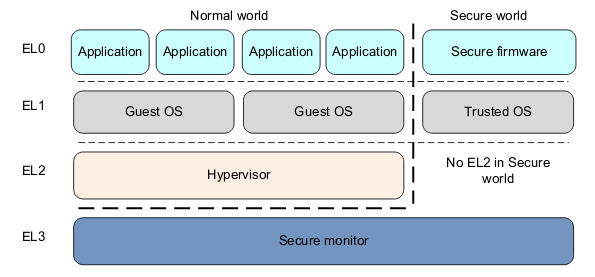
\includegraphics[scale=0.6]{tesi7.png}
\caption[ARMv8 Exception Levels]{ARMv8 Exception levels and their main purpose}\label{fig:armv8el}
    \end{center}
\end{figure}

We describe briefly the function of each exception level:
\begin{description}
    \item[EL0] is the lowest exception level, often referred to as ``unprivileged''
        in opposition to every other, ``privileged'', level. It has severe 
        limitation in accessing system registers and failure to respect them
        is met with a synchronous abort. It is meant to run user application, 
        processes below the kernel.
    \item[EL1] is the first privileged level. It is where most interrupts end
        up and is meant for the OS kernel.
    \item[EL2] is the Hypervisor level; here resides harware support for virtualization,
        a level meant to supervise virtual machines. For example, KVM is an in-kernel
        virtualization running at level \textbf{EL2} and supervising the virtual kernel 
        at \textbf{EL1}.
    \item[EL3] is used to separate the system into secure partitions with the
        hardware TrustZone support.
\end{description}

\subsection{Changing Exception Level}
A change in the current exception level can be either caused by a willing decision
of a higher privilege \textbf{EL} to a lower privilege \textbf{EL} or following 
an exception. Moreover, an exception cannot be taken to a lower exception level (e.g. if the core 
is currently at \textbf{EL2} and an interrupt line that should be handled
at \textbf{EL1} is asserted it will be ignored as long as the exception
level is not lowered, regardless of interrupt enabling). 
To access a lower exception level an {\tt eret} instruction is required: {\tt eret}
loads the state stored in \textbf{SPSR\_ELn} (see \ref{spsr}), where \textbf{ELn} 
is the current exception level, as the new system status (exception level included).
Since no exception ever handled at \textbf{EL0}, \textbf{EL0} is only reachable 
on {\tt eret} instructions.

Exceptions are normally taken to \textbf{EL1} but can be set to run in \textbf{EL2}
or even \textbf{EL3} by configuring corresponding system registers \textbf{HCR\_EL2}
and \textbf{SCR\_EL3}, Hypervisor Configuration Register and Secure Configuration
Register respectively. 

It is also possible to change execution \textit{state} (i.e. AArch64 or AArch32)
during runtime, but that is irrelevant for the scope of this work, that lies
entirely in AArch64.

\section{Registers}
\subsection{General Purpose Registers}
One of the immediate benefits of 64 bit architecture is a larger register pool:
ARMv8 uses 31 64-bits wide general purpose registers, more than doubling from
ARMv7.
The registers are numbered from \textbf{x0} to \textbf{x30}. Although they are
freely accessible the developer should be mindful of their secondary purpose
for function calling convention (both C and Assembler):
\begin{itemize}
    \item \textbf{x0} to \textbf{x7} are used to hold both arguments and return
        value (only \textbf{x0}) of a C function.
    \item \textbf{x8} is used to pass an indirect result value (e.g. a returned 
        structure, in which case x8 holds the address to a properly set memory
        location).
    \item \textbf{x9} to \textbf{x18} are used to hold local variables in a 
        routine call. They are caller-saved, which means that it is the caller
        responsibility to preserve their content before issuing a C function call.
    \item \textbf{x19} to \textbf{x28} are similar temporary registers, but for 
        the callee to restore before returning; they are referred as callee-saved.
    \item \textbf{x29} is the frame pointer.
    \item \textbf{x30} is the link register.
\end{itemize}
Every general purpose register also has a 32 bit alias obtained replacing ``x''
with ``w'' in the register's name (from \textbf{w0} to \textbf{w30}) that permits
access to the lower (i.e. least significant) 32 bits of the register; the upper 
32 bits are ignored.

\begin{figure}[h]
    \begin{center}
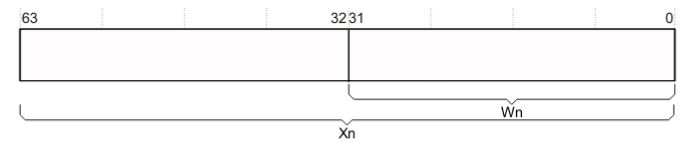
\includegraphics[scale=0.55]{tesi8.png}
\caption[32 bit alias]{64 bit register with ``x'' and ``w'' access}\label{fig:32reg}
    \end{center}
\end{figure}

\subsection{Special Registers}
\label{spsr}
There are 5 special registers:
\begin{description}
    \item[Zero Register:] \textbf{xzr} and \textbf{wzr} provide access (as 64 and
        32 bit register respectively) to a special register that ignores write
        attempts and always read as zero.
    \item[Program Counter (pc):] up until ARMv7 the program counter was a general purpose
        register held in \textbf{r15}. In ARMv8 it has a very limited access,
        being read only and only implicitly used in certain instructions. This is 
        one of the biggest differences with previous architecture and caused a 
        lot of initial confusion; its restrictiveness results nonetheless in a
        much clearer and less error prone program flow.
    \item[Exception Link Register (elr):] without free access to the program counter
        the system must provide an alternative way to restore a process' execution
        point. The exception link register holds the exception return address: it 
        is automatically filled when one is fired and can be overwritten. Upon
        executing an {\tt eret} instruction the value in \textbf{elr} is set as the
        program counter.
    \item[Saved Process Status Register (spsr):] similarly to \textbf{elr}, this
        register is automatically initialized with various status informations
        upon taking and exception, and is restored (after eventual modification)
        with an {\tt eret} instruction.
    \item[Stack Pointer (sp):] The current stack pointer. It is freely accessible
        both in read and write operations.
\end{description}

\begin{figure}[t]
    \begin{center}
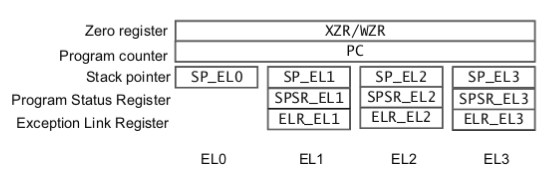
\includegraphics[scale=0.68]{tesi9.png}
\caption[special registers]{AArch64 special registers}\label{fig:specialreg}
    \end{center}
\end{figure}

As depicted in figure \ref{fig:specialreg} some special registers have different
versions for different exception levels: there is a separated stack pointer 
for all four of them and \textbf{EL0} is the only level missing \textbf{spsr}
and \textbf{elr} (owing to the fact that they are exception related registers, and
\textbf{EL0} never deals with exceptions or {\tt eret} instructions).

Access to a special register from a different exception level is permitted if 
said register belongs to a lower level: for example \textbf{EL3} can set all the
other stack pointers (including its own), but \textbf{EL1} trying 
to do the same will trigger an abort for \textbf{sp\_el2} and \textbf{sp\_el3}.

\subsection{System Registers}
Another significant turn from ARMv7 is the absence of a coprocessor interface.
A coprocessor is an auxiliary core used to supplement the functions of the primary
processor; ARMv7 specified a generic coprocessor interface to connect up to 
15 assisting cores, of which one was reserved for system registers management.
While coprocessors had to be controlled via specific instructions ARMv8 system registers
are directly accessed in Assembly with the {\tt mrs} and {\tt msr} instructions
as per any other register. This is a welcome change that simplifies the developer's
approach to system configuration.

Similarly to special registers many system registers have different, banked versions
for some or all exception levels (usually not \textbf{EL0}), each with the
suffix \textit{\_ELn} to indicate the corresponding level.
There registers are usually 32 bits wide. What follows is a list of system registers
considered most important for the purpose of this work; for a detailed description
of the various bit fields refer to the ARM reference manual \cite{armarm}.
\begin{description}
    \item[Exception Syndrome Register:] \textbf{ESR\_EL\textit{n}}, for each exception 
        level holds the information regarding the last occurred exception (only
        for synchronous and SError, not for IRQs and FIQs. See \ref{exceptions}
        for more on exceptions). It is necessary to distinguish between exception
        classes and to find details specific to the exception.
    \item[Fault Address Register:] \textbf{FAR\_EL\textit{n}}, it is used in pair 
        with \textbf{ESR\_EL\textit{n}} to find which address caused a Data or 
        Instruction synchronous abort.
    \item[Hypervisor Configuration Register:] \textbf{HCR\_EL2}, controls 
    virtualization settings and trapping of exceptions to \textbf{EL2}.
    \item[Memory Attribute Indirection Register:] \textbf{MAIR\_EL\textit{n}}, 
        stores the user-provided memory attribute encodings corresponding to the
        possible values in a MMU translation table entry for translations at level \textit{n}.
    \item[Multiprocessor Affinity Register:] \textbf{MPIDR\_EL1} is the 
        executing core id, used mainly to distinguish on which core the code is 
        runnint on.
    \item[Secure Configuration Register:] \textbf{SCR\_EL3} controls Secure 
    state and trapping of exceptions to EL3.
    \item[System Control Register:] \textbf{SCTLR\_EL\textit{n}} controls 
    architectural features, for example the MMU, caches and alignment checking.
    \item[Translation Table Base Register 0:] \textbf{TTBR0\_EL\textit{n}}, holds
        the address to the MMU translation table used normally at each exception level.
    \item[Translation Table Base Register 1:] \textbf{TTBR1\_EL1}, holds
        the address to the a special translation table used to separate application
        and kernel space. See section \ref{mmu} for more.
    \item[Vector Based Address Register:] \textbf{VBAR\_EL\textit{n}} is a pointer 
        to the exception vector table for level \textit{n}.
\end{description}

\subsection{PSTATE}
A reader with experience in ARM architecture will surely notice the lack of a
current program status register, holding informations like the current exception
level, aritmetic flags, interrupt mask and so on.
The AArch64 version of said register is implicitly present and not directly 
accessible. Instead, the single fields are supplied to read and
write independently; this collection of ``fake registers'' is globally called 
\textbf{PSTATE}. Curiously, querying for the \textbf{CPSR} register in a GDB 
debugger will correctly display the \textbf{PSTATE} components as a whole, although
no such register can be loaded from or stored to in Assembly code.

\begin{table}[t]
    \begin{center}
    \begin{tabular}{|c|c|c|}
    \hline
    \rowcolor[HTML]{9B9B9B} 
    Field name & Register handle              & Description                                                                                                                                                                                           \\ \hline
    N          & \cellcolor[HTML]{FFFFFF}None & Negative condition flag                                                                                                                                                                               \\ \hline
    Z          & None                         & Zero condition flag                                                                                                                                                                                   \\ \hline
    C          & None                         & Carry condition flag                                                                                                                                                                                  \\ \hline
    V          & None                         & Overflow condition flag                                                                                                                                                                               \\ \hline
    D          & daifset and daifclr          & Debug mask bit                                                                                                                                                                                        \\ \hline
    A          & daifset and daifclr          & SError mask bit                                                                                                                                                                                       \\ \hline
    I          & daifset and daifclr          & Interrupt mask bit                                                                                                                                                                                    \\ \hline
    F          & daifset and daifclr          & Fast interrupt mask bit                                                                                                                                                                               \\ \hline
    SS         & None                         & Software Step bit                                                                                                                                                                                     \\ \hline
    EL         & CurrentEl                    & Current exception level                                                                                                                                                                               \\ \hline
    nRW        & None                         & \begin{tabular}[c]{@{}c@{}}Current execution state\\ (AArch32 or AArch64)\end{tabular}                                                                                                                \\ \hline
    SP         & None                         & \begin{tabular}[c]{@{}c@{}}Stack pointer selector\end{tabular} \\ \hline
    \end{tabular}
    \caption[PSTATE fields]{PSTATE fields definitions}
\end{center}
    \end{table}

\section{Exception Handling}
In ARM architecture exceptions are conditions or system events that require some 
action by privileged software to ensure smooth 
functioning of the system; said condition is taken care of immediatly by interrupting
the normal flow of software execution and starting another routine (the exception
handler).
There are several classes of exceptions; every class can branch in different kinds,
and every exception can be either synchronous or asynchronous (see figure \ref{fig:exceptions}).

The code to run when an exception is fired is specified by the developer in an 
exception vector table. The pointer to the exception vector table is written to 
\textbf{VBAR\_EL\textit{n}} register, for \textit{n} ranging from level 1 to 3,
so every exception level has its own table (nothing prevents multiple levels
to point to the same table however). For exceptions fired while at \textbf{EL0} 
the table for \textbf{EL1} is used.

The exception table can be anywhere in memory but must be 128 bytes aligned and 
must have the format specified in table \ref{etable}.
Each entry in the table is 16 instructions long, allowing for some control logic 
to be present in the top level handler as well, before branching to a more complex
routine.
The table can be divided in four sections:
\begin{enumerate}
    \item handlers to be used when the exception does not change neither the current 
        exception level nor the stack pointer.
    \item handlers to be used when the exception does not change the current 
        exception level but should use a specific stack pointer.
    \item handlers to be used when the exception elevates the privilege level and
        the execution state is in AArch64.
    \item handlers to be used when the exception elevates the privilege level and
        the execution state is in AArch32.
\end{enumerate}

Each section has four different handlers for synchronous exceptions, IRQ, FIQ
and SError.

\begin{table}[t]
    \begin{center}
    \begin{tabular}{|l|l|l|}
    \hline
    \rowcolor[HTML]{9B9B9B} 
    Address           & Exception type & Context                                                                            \\ \hline
    VBAR\_ELn + 0x00  & Synchronous    &                                                                                    \\ \cline{1-2}
    VBAR\_ELn + 0x80  & IRQ/vIRQ       &                                                                                    \\ \cline{1-2}
    VBAR\_ELn + 0x100 & FIQ/vFIQ       &                                                                                    \\ \cline{1-2}
    VBAR\_ELn + 0x180 & SError/vSError & \multirow{-4}{*}{\begin{tabular}[c]{@{}l@{}}Current EL\\ with SP0\end{tabular}}    \\ \hline
    VBAR\_ELn + 0x200 & Synchronous    &                                                                                    \\ \cline{1-2}
    VBAR\_ELn + 0x280 & IRQ/vIRQ       &                                                                                    \\ \cline{1-2}
    VBAR\_ELn + 0x300 & FIQ/vFIQ       &                                                                                    \\ \cline{1-2}
    VBAR\_ELn + 0x380 & SError/vSError & \multirow{-4}{*}{\begin{tabular}[c]{@{}l@{}}Current EL\\ with SPx\end{tabular}}    \\ \hline
    VBAR\_ELn + 0x400 & Synchronous    &                                                                                    \\ \cline{1-2}
    VBAR\_ELn + 0x480 & IRQ/vIRQ       &                                                                                    \\ \cline{1-2}
    VBAR\_ELn + 0x500 & FIQ/vFIQ       &                                                                                    \\ \cline{1-2}
    VBAR\_ELn + 0x580 & SError/vSError & \multirow{-4}{*}{\begin{tabular}[c]{@{}l@{}}Lower EL\\ using AArch64\end{tabular}} \\ \hline
    VBAR\_ELn + 0x600 & Synchronous    &                                                                                    \\ \cline{1-2}
    VBAR\_ELn + 0x680 & IRQ/vIRQ       &                                                                                    \\ \cline{1-2}
    VBAR\_ELn + 0x700 & FIQ/vFIQ       &                                                                                    \\ \cline{1-2}
    VBAR\_ELn + 0x780 & SError/vSError & \multirow{-4}{*}{\begin{tabular}[c]{@{}l@{}}Lower EL\\ using AArch32\end{tabular}} \\ \hline
    \end{tabular}
    \caption[Exception table]{Exception table format}
    \label{etable}
\end{center}
    \end{table}

\subsection{Interrupts}
Interrupts can be fast interrupts (FIQ) or normal interrupts. Aside from the fact 
that FIQ have higher priority, these two types of exception are virtually identical.
Usually it is the developer's responsibility to route an interrupt source to 
IRQ or FIQ.
Interrupts are tipically associated with external hardware and connected to 
input pins to the core. The connection can be direct or, more commonly, pass through
an external device called interrupt controller that elaborates interrupt priorities
and organization (see section \ref{gic}).

Because the occurrence of interrupts is not directly related to the instruction
cycle being executed by the core at any given time, they are classified as
asynchronous exceptions.

 \begin{figure}[t]
 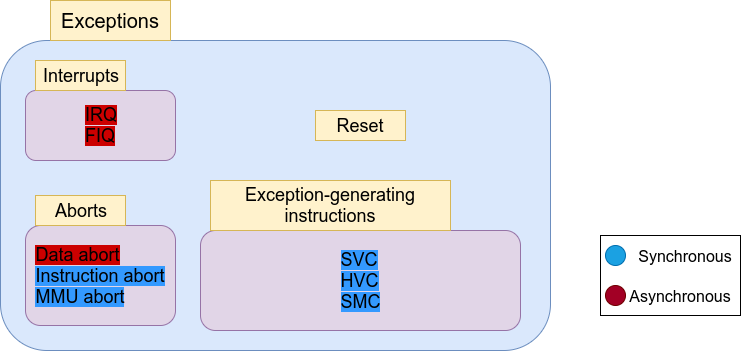
\includegraphics[scale=0.525]{tesi10.png} 
 \caption[Exceptions]{Tree of exception classes.}\label{fig:exceptions}
 \end{figure}

%TODO: add a diagram

\subsection{Aborts}
Abort exceptions, also called system errors (SError), occur every time some abnormal
condition is met during a memory access. Instruction Aborts result from an error
during an instruction fetch cycle, while Data Aborts follow failed data access.

Despite the names depicting error conditions, aborts can work in perfectly normal
and predictable flows. This is the case of MMU faults, generated by the Memory
Manage Unit on occasions like access to dirty page entries.
The severity of conditions that set off abort exceptions can be configured to 
some extent with system registers; for example, a TLB miss can be ignored or 
fire an exception, and memory accesses can pass through address alignment 
and permission checks which may or may not interrupt the process.

Aborts can be both synchronous and asynchronous. MMU faults and alignment induced 
aborts are always synchronous, while data aborts can be asynchronous in certain
situations.

\subsection{Reset}
Reset is a special exception, fired on power up of the processor. Its handler is 
implementation-specific and presumably located at address {\tt 0x80000} in the 
case of the BCM2837.

\subsection{Exception Generating Instructions}
We have seen that a core can lower its exception level with {\tt eret}, but can
only increase it through an exception. For this purpose there are Assembly instructions
that induce an exception to a higher exception level, usually to require a service 
paired with an higher privilege. The most obvious example of this behaviour are
system calls.
\begin{itemize}
    \item \textbf{SVC:} the supervisor call instruction fires an exception
        handled at \textbf{EL1}. Used by user programs to require kernel services.
    \item \textbf{HVC:} the hypervisor call instruciton fires an exception
        handled at \textbf{EL2}. Used by the guest OS to require hypervisor services.
    \item \textbf{SMC:} the secure monitor call instruction fires an exception
        handled at \textbf{EL3}. Allows to require \textit{secure world} context
        switch.
\end{itemize}
Since those exceptions follow an instruction execution they are by definition
synchronous.

\section{Memory Attributes}
\label{mair}

\section{Multiprocessor}

\section{Security}

\section{ARM Timer}

\clearpage{\pagestyle{empty}\cleardoublepage}
\chapter{The Memory Management Unit}
The Memory Management Unit is a device found in most CPUs tasked with the objective
of translating virtual memory addressing with physical addressing. The Cortex-A53
is no exception and has an advanced internal MMU. It is such an important part
of the system that even if it's technically part of the ARMv8 specification it 
deserves a chapter on its own.

The main purpose of address translation is to allow each process to have its own
virtual address space that has nothing to do with how much memory is available 
(and where this memory is located) on the system, with hardware MMIO and other
processes hidden from its view.
If the memory management unit is active any address used in the system is first
elaborated and translated: different sections of the 64 bits address (starting
from most significant ones) are used to index different levels of a tree containing
translation entries. Then there can be additional checks on whether the current
exception level has the proper permissions to access the resulting physical memory.
Only then the actual access is performed; all of this is handled by the hardware and 
can be almost entirely ignored by the programmer after setup.

\section{Address Translation}
As briefly mentioned in the introduction when the MMU is active every address is 
treated as multiple indexes for the translation table. The translation table is 
a tree of translation entries that map a section of RAM: each level of the 
tree has entries covering a certain number of elements in the next level until the 
last, that maps memory directly.

The following example considers a tree where each entry before last level
points to 512 more entries and 
depicts a trivial ``identity'' mapping: every virtual address is translated in 
the same physical address. The bottom level covers a 4KiB block of memory directly
(this reason for these numbers will be explained in section \ref{translationsize}). There
are four levels in the tree, level 0 to 3.
Presume we want to translate a 64 bits address:
\begin{itemize}
    \item the 16 most significant bits are reserved for kernel space virtualization
        (more on this topic in section \ref{kernelvirt}).
    \item bits 47:39 are the level 0 table and reference a level 1 entry. Each
        level 0 entry spans a 512 GiB memory range ($2^39$).
    \item bits 38:30 are the level 1 table and reference a level 2 entry. Each
        level 1 entry spans a 1GiB memory range ($2^30$ or $512 GiB / 512$).
    \item bits 29:21 are the level 2 table and reference a level 3 entry. Each
        level 2 entry spans 2 MiB memory range, similarly to previous levels.
    \item bits 20:12 are the level 3 table and reference the last level, made of 
        direct memory blocks. Each memory block is 4KiB wide.
    \item bits 12:0 are the offset for the last memory block and index the actual
        word referenced.
\end{itemize}

%TODO:immagine

In this mundane example it is evident how the translation process is arbitrary;
every level can simply be cut off and the resulting address be obtained by adding
the intermediate indexes and the remaining bits (to be considered as the final 
offset). This is not possible anymore if the translation function is not an 
identity. 
In this case the translation function is codified by the pointers in the table entries;
the table entry marks the beginning of the next level of tables and the corresponding
piece of virtual address indexes the chosen entry.

\subsection{Granule Size}
\label{translationsize}
With granule size we refer to the smallest possible block of memory that can be 
indexed by the MMU tables; in the previous example, 4KiB.
The ARMv8 specification allows for three different granule sizes: 4KiB, 16KiB and 64KiB.
The actual ARM processor abiding to the standard can in turn implement those granules
only partially. The Cortex-A53 implements them all.
The granule size is a global setting, affecting the entirety of the page table.
Different granule size dictate how many levels is possible to have and how many
entries are in each table (for example, a granule of 64 KiB allow only 3 levels
and a granule of 16KiB will result in 10 bit wide address sections).

A small granule size will result in more control but also in a bigger table; to 
divide a 2GiB RAM into 4KiB blocks an operating system will need 524288 64 bits
wide table entries, for a total of 4MiB of allocated memory.
Choosing a fine grained control does not mean commiting to it, however. If there
are large sections of memory with the same memory attributes and virtual addressing
(e.g. MMIO memory that should generally not be accessed by user processes) the 
developer can ``cut early'' the page table tree and use any intermediate memory
range. In the above example we could arbitrarily stop at level 2 and create a part
of the table with direct entries spanning 2 MiB each.

%TODO: immagine

\section{Table Descriptor Format}
When in AArch64 there is a single accepted format for table entries. We will now
consider the configuration consequential to a 4 KiB granule size; other choices
differ sligtly in translation indexes width and position, but maintain the same
core concepts. The table descriptor is 64 bits wide, separated in fields like 
in figures \ref{fig:desc1} and \ref{fig:desc2}.

Any table entry is one of two types:
\begin{enumerate}
    \item \textbf{A table descriptor} that points to another table entry in the 
        next level.
    \item \textbf{A block entry} that resolves directly into a memory range of 
        variable size, depending on the level.
\end{enumerate}

The entry type is defined by the two least significant bits in the descriptor, 
as depicted in table \ref{tab:desc}; an invalid entry leads to an MMU fault exception.
Note that not every level can host a block entry; with a granule size of 4 KiB, 
level 0 does not admit that kind of descriptor.

\subsection{Table Descriptors}
Table descriptors point to a table entry in the next level. Bit fields have the 
following meaning:
\begin{itemize}
    \item \textbf{[0]} marks the validity of the entry; 1 is valid, 0 is invalid.
    \item \textbf{[1]} is the entry type. It is 1 for table next level descriptors.
    \item \textbf{[2:11]} are ignored/reserved bits.
    \item \textbf{[12\footnote{\label{4knote} This value can be different for granule
        sizes other than 4KiB}:47]} is the address of the next level table. It is codified
        as if it started from the least significant bit, with 
        [11\footnote{see footnote \ref{4knote}}:0] bits assumed
        as 0. Because of this all page tables must be 4096 ($2^12$) bytes aligned.
    \item \textbf{[48:58]} are ignored/reserved bits.
    \item \textbf{[59]} PXNTable field: private execute never bit for subsequent
        levels of lookup; if set the memory range covered by this and following entries
        cannot be executed by code at level \textbf{EL0}.
    \item \textbf{[60]} XNTable field: execute never bit for subsequent levels
        of lookup; if set the memory range covered by this and following entries
        cannot be executed.
    \item \textbf{[61:62]} APTable field: access permission bits for subsequent levels
        of lookup; this field enforces permission rules for the memory range
        indexed by this and following entries, combined in a hierarchical 
        fashion (see table \ref{tab:aptable}). Subsequent table entries can
        further restrict the permission rules but cannot loosen them; failure
        to heed said rules will result in an appropriate abort exception.
    \item \textbf{[63]} NSTable field: when in secure state this bit specifies
        the security state for subsequent levels of lookup. When not in secure state
        it is ignored.
\end{itemize}

\begin{table}[h]
    \begin{center}
    \begin{tabular}{|c|l|}
    \hline
    \rowcolor[HTML]{9B9B9B} 
    \multicolumn{1}{|l|}{\cellcolor[HTML]{9B9B9B}APTable{[}1:0{]}} & Restriction                                                                                                                                            \\ \hline
    00                                                             & No effect on subsequent levels of lookup                                                                                                               \\ \hline
    01                                                             & \begin{tabular}[c]{@{}l@{}}Any access to this memory range from EL0\\ is forbidden.\end{tabular}                                                       \\ \hline
    10                                                             & Memory is read-only.                                                                                                                                   \\ \hline
    11                                                             & \begin{tabular}[c]{@{}l@{}}Any access to this memory range from EL0\\ is forbidden, while it is read-only for\\  higher privilege levels.\end{tabular} \\ \hline
    \end{tabular}
    \label{tab:aptable}
    \caption[APTable]{Access Permission Table bit fiels. The two bits can be 
    separated and seen as read-only bit ([0]) and \textbf{EL0} access ([1])}
\end{center}
\end{table}

%TODO: immagine fig:desc1

\subsection{Block Descriptors}
Block descriptors represent direct access to a block of memory; when one is reached,
it is the last stage of the translation process. They contain the following bit
fields:
\begin{itemize}
    \item \textbf{[0]} marks the validity of the entry; 1 is valid, 0 is invalid.
    \item \textbf{[1]} is the entry type. It is 0 for block descriptors.
    \item \textbf{[2:4]} memory attributes index field. The value found here
        indexes a memory address configuration defined in corresponding 
        the \textbf{MAIR\_EL\textit{n}} register (see section \ref{mair}).
    \item \textbf{[5]} is the non-secure bit. For memory accesses from 
        secure state specifies whether the output address is in
        the secure or non-secure address map. For accesses from non-secure state
        this bit is ignored.
    \item \textbf{[6:7]} are data access permission bits. Similar to APTable bits,
        they are referred to the immediate block of memory (and can be further
        restricted by previous APTable settings). For possible values see table
        \ref{tab:apbits}.
    \item \textbf{[8:9]} sets the shareability of the memory block, configuring
        caching capabilities.
    \item \textbf{[10]} is the access flag (AF). If it is not set it means the 
        selected entry is accessed for the first time, in which case an MMU abort
        will be fired. The exception handler should take care of the initialization,
        set the access flag to 1 and attempt again the memory access.
    \item \textbf{[11]} is the not global bit (nG). If a lookup using this 
        descriptor is cached in a TLB, determines whether the TLB
        entry applies to all ASID values, or only to the current ASID value
        (see section \ref{tlb} for more).
    \item \textbf{[12:47]} is the address to the memory block that is pointed byte
        the descriptor. It is aligned similarly to the address in a table descriptor,
        but it contains actual memory instead of a next level page table.
    \item \textbf{[48:50]} are ignored/reserved bits.
    \item \textbf{[51]} is the Dirty Bit Modifier (DBM), and it is used to keep
        track of differences between caches and real memory. If it is set, caches
        should be checked for stale entries. It can be managed either via 
        hardware or software.
    \item \textbf{[52]} is the Contigous bit, a hint bit indicating that the 
        translation table entry is one of a contiguous set or entries and may be
        be cached in a single TLB entry.
    \item \textbf{[53]} PXN bit: privileged execute never bit. If set, the memory block's 
        execution at unprivileged exception levels (\textbf{EL0}) is forbidden.
    \item \textbf{[54]} XN bit: execute never bit. If set, the memory block's 
        execution is forbidden.
    \item \textbf{[55:63]} are ignored/reserved bits.
\end{itemize}

\begin{table}[]
    \begin{center}
    \begin{tabular}{|l|l|l|}
    \hline
    \rowcolor[HTML]{9B9B9B} 
    AP{[}2:1{]} & Access from privileged EL & Access from EL0 \\ \hline
    00          & Read and write            & Forbidden       \\ \hline
    01          & Read and write            & Read and write  \\ \hline
    10          & Read-only                 & Forbidden       \\ \hline
    11          & Read-only                 & Read-only       \\ \hline
    \end{tabular}
    \caption[APBits]{Access Permission Bits values. similarly to \ref{tab:aptable},
    the two bits 1 and 0 can be interpreted separately as write restriction for higher
    exception level and access for \textbf{EL0}, respectively.}
    \label{tab:apbits}
\end{center}
    \end{table}

%TODO: immagine fig:desc2

\section{Kernel Space Virtualization}
\label{kernelvirt}
In a tipical OS environment multiple processes run concurrently and use dynamically
allocated memory and resources. The memory management unit serves to this purpose:
every process have its own set of translation tables managed by the kernel and sees a 
contiguous range of memory at its disposal. In this multitude of actors we can
consider the kernel as a process in its own right, albeit of a superior kind; because
it has no peers and often uses a static memory space the translation mechanism
is meaningless, if not cumbersome, for him.

To fix this situation the ARMv8 provides a number of features. One may intuitively
imagine different page table references for each Exception Level, but this is 
only partially the case. \textbf{EL0} and \textbf{EL1}, the main levels of operation
for user processes and kernel, share in fact the same page table register 
(\textbf{TTBR0\_EL1}): the register used to properly divide user and kernel pages 
is \textbf{TTBR1\_EL1}. Like the latter, it holds the base address of a page table;
while \textbf{TTBR0\_EL1} is used with any normal address resolution,
 \textbf{TTBR1\_EL1} is selected when 16 most significant bits of the address 
 are set to one, forming an address that would be absurdely big for any memory 
 designed in the foreseeable future.

 The kernel can then operate in this virtual memory range with a personal page
 table (possibly as an identity transformation) while normal processes live in 
 lower addresses of virtual memory. To accomodate the kernel in this inexistent
 range the addresses in its code must be set properly. This would requires either
 a linker script instructing to compile for memory starting at 
 {\tt 0xFFFF00000000000000} (in which case the MMU must be configured and 
 enabled immediatly) or compiling the code for relative branch instructions only.
 The latter approach is considered easier as it works even if the MMU is disabled
 and only requires the kernel entry point (the exception table) to be tweaked 
 when address translation is eventually turned on.

 As a side note, the condition to select the \textbf{TTBR1\_EL1} register can
 be limited to the second most significant byte of the address set to {\tt 0xFF};
 the first byte can then be freely used by the kernel software for personal 
 purposes.

 \begin{figure}[h]
 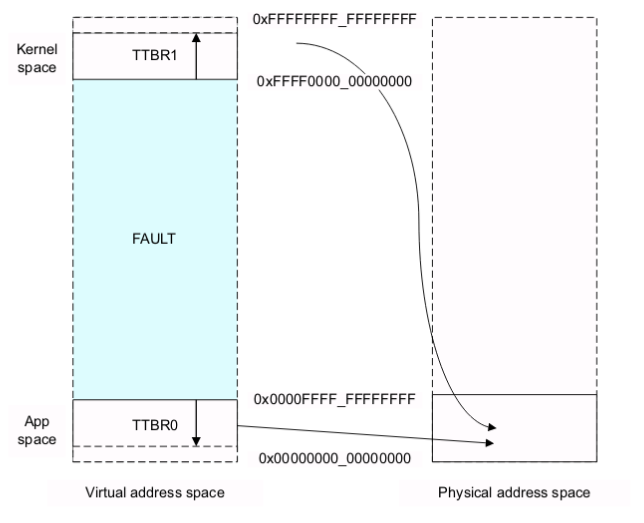
\includegraphics[scale=0.6]{tesi11.png} 
 \caption[Kernel memory virtualization]{In this image kernel and user spaces 
 are positioned at the opposites of the address range but both are mapped in 
 the same physical area.}\label{fig:exceptions}
 \end{figure}
 %16 ExbiByte


 An example use case might be in support of object-oriented programming languages:
 as well as having a pointer to an object, it might be necessary to keep a 
reference count that keeps track of the number of references or pointers or handles
 that refer to the object, for example, so that automatic garbage collection 
 code can deallocate objects that are no longer referenced. This reference 
 count can be stored as part of the tagged address rather than in a separate table, 
speeding up the process of creating or destroying objects.

\subsection{EL2 and EL3 Translation Process}
The virtualization and secure levels have their own page tables. Since they act
as overlay for one or more guest operating systems when enabled there are two translation
stages: the first one is performed by the OS, using \textbf{TTBR\textit{n}\_EL1}
as already explained; the result from this stage is then fed to a second stage,
using tables found in \textbf{TTBR0\_EL2} and \textbf{TTBR0\_EL3}.

Such complex tools are out of the scope of this work.


\section{Translation Lookaside Buffer}
\label{tlb}
The Translation Lookaside Buffer (or TLB) is simply cached memory for address translation
results: when a virtual address is to be translated the TLB is checked first;
if the address is found (TLB hit) then the cached value is used. If not (TLB miss)
a page table walk is performed and the result is stored in the TLB. Alternately,
an MMU fault can be configured to fire.

The TLB and MMU intertwined operation works very differently in ARM compared to 
MIPSEL architecture and with an arguably easier approach for a novice. The TLB 
component activity is almost invisible to the OS developer not caring for 
particular performance optimizations, so it can be safely ignored. The only 
essential part is the configuration of proper page tables for each process.

\subsection{Trivial Approach}
Once the MMU is activated and page tables are initialized the kernel must make 
sure every process can only see its virtual memory share during its designated
time slice. This can be achieved by creating a different page table per process
and simply substituting it completely every time there is a context switch.
A problem presents when a process asks for the same virtual address, that should
however be translated in a different physical address, of one of its peers; 
we shall call them process \textit{a} and \textit{b}.
If the entry relative to \textit{a} is found in the TLB by \textit{b} its value
will be returned without performing a page table walk, and will result in the
wrong memory being accessed.

Without delving too deeply into MMU operation, a simple solution will be to 
flush the TLB cache every time there is a context switch. This will effectively
deny most of the optimization brought by the cache, but will also prevent
incorrect translations.

\subsection{ASID Approach}
A more elegant and efficient solution consists in using an Address Space ID (ASID)
to keep track of process property in TLB entries. The ASID is arbitrarily assigned
to processes by the kernel and stored in the two most significant bytes of either
\textbf{TTBR0\_EL1} or \textbf{TTBR1\_EL1}
When the non-global (\textit{nG}) field of a block entry in the page table is 
set the current ASID is saved alongside the address in a TLB entry. Subsequent
lookups for that address in the TLB cache only match if both the address and the
saved ASID correspond to present values.

% TODO: remember ttbcr; eventually describe MMU register configuration in greater
% detail


\clearpage{\pagestyle{empty}\cleardoublepage}
\chapter{Overview of the BCM2837}
The BCM2837 is the System-on-Chip produced by Broadcom that is used for most
of the Raspberry Pi family of boards, and for the third version specifically.
 Some of them are built with variants like BCM2836 (for the Rasbperry Pi 2)
  and BCM2835 (the first used, for the Raspberry Pi 1): the scarce documentation
  is only available for BCM2835 \cite{bcm2835} (and partly for BCM2836 \cite{rev3.4})
  allegedly because nothing changes from the developer perspective; the actual 
  differences have been figured out mostly through reverse engineering from the 
  code of the various Linux distributions.

The BCM2837 contains the following peripherals, accessible by the on-board ARM CPU:
\begin{itemize}
    \item A system timer.
    \item Two interrupt controllers.
    \item A set of GPIOs.
    \item A USB controller.
    \item Two UART serial interfaces.
    \item An external mass media controller (the microSD interface).
    \item Other minor peripherals (I2C, SPI,\ldots).
\end{itemize}

\section{Boot Process}
As is the case for many similar boards the ARM CPU is not the main
actor, but actually more of a coprocessor for the Videocore IV GPU installed
alongside it.

On reset the first code to run is stored in a preprogrammed ROM chip read by the GPU,
called the first-stage bootloader. This first bootloader looks for the first
partition on the microSD card (which has to be formatted as FAT32), mounts
it and loads (if present) a file called bootcode.bin from the partition.
This binary is part of the Broadcom proprietary firmware package, and is considered
the second-stage bootloader.
At this point of the boot sequence the RAM is still not initialized, so the second-stage
bootloader is run from the L2 memory cache. This firmware initializes the RAM 
and in turn loads on it another file from the microSD card, start.elf.
Another firmware for the Videocore, start.elf has the responsibility to split 
the RAM in two parts for the GPU and the CPU; after that it reads the config.txt 
file (if present) and loads its parameters starting at address 0x100.
 Finally it does the same with the kernel image and passes control to the ARM CPU.

 \begin{figure}[t]
 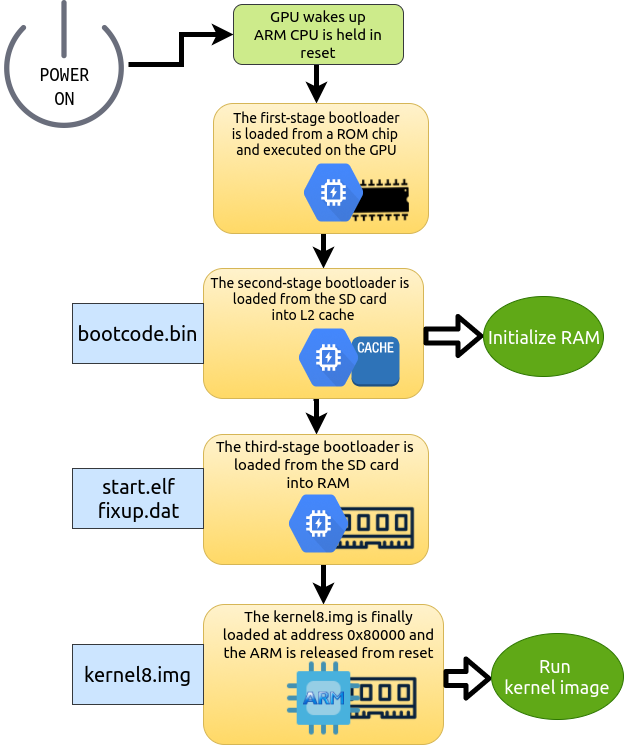
\includegraphics[scale=0.6234]{tesi1.png}
 \caption[Figure 1]{Explanatory diagram on BMC2837 boot sequence}\label{fig:prima}
 \end{figure}
 \clearpage
%TODO: add a diagram

Every step up until the loading of the kernel image in memory is handled by 
the GPU and can be safely ignored after an initial setup.

\subsection{MicroSD Contents}
The microSD must have its first partition formatted as FAT32; there are no 
further restrictions on following partitions. The absolute bare minimum contents 
are just four files:
\begin{enumerate}
    \item \textbf{bootcode.bin}: second-stage bootloader, necessary for the GPU
            to load the third-stage bootloader.
    \item \textbf{start.elf}: third-stage bootloader, necessary for the GPU to load
            the kernel image in RAM.
    \item \textbf{fixup.dat}: a file containing relocation data to be referenced 
            by start.elf when loading into RAM; This allows for the same firmware 
            to be used for all versions of the Raspberry Pi, which range in 
            memory from 256MB to 1GB. If not included the board might still boot,
            but it will likely only report a total of 256MB regardless of the
            actual installed RAM.
    \item \textbf{kernel8.img}: kernel binary for the ARM CPU.
\end{enumerate}
Of those four files only the kernel image is user provided; the remaining firmware
is distributed and updated in compiled form by the Raspberry Pi foundation with
proprietary licensing from Broadcom.

\subsection{Configuration}
It is possible to configure in different ways the boot process by combining
different firmware binaries and config.txt options, but this work always uses
the default with no extra steps needed; this is to ensure the usage is kept
as simple as possible and since the base behaviour never presented any issue.
Of all the available options, only the following two were ever considered 
(but still never implemented).

\subsubsection{Architecture}
The Cortex A-53 can run both ARM32 and ARM64 code; the choice is dictated by the
name of the kernel image: {\tt kernel8.img} makes the CPU start in AArch64 mode,
while {\tt kernel7.img} would start in AArch32.

\subsubsection{Kernel Loading Address}
The GPU loads the kernel image starting at address 0x80000 in RAM for the
Raspberry Pi 3. By adding a config.txt file to the microSD card and using
the kernel\_address parameter the image file will be loaded at the specified
starting point. Similarly, by setting the kernel\_old parameter to 1 the binary
will be loaded at the beginning of the main memory, at address 0x0.

Although these options can bring a more clean memory disposition, it was decided
the advantages were not worth adding an additional file to the necessary setup.
Additionally, while the Raspberry Pi harware correctly interprets these commands
the Qemu emulated machine is not entirely loyal to reality and actively resists
any attempt to move the kernel to locations other than 0x80000 (more details can
be found in chapter 7).

\subsubsection{Memory Split}
As previously mentioned the two main actors on the BCM2837, the quadcode Cortex-A53 ARM
and the Videocore IV GPU, share the same 1GiB RAM space. Without other instruction
the start.elf bootloader fixes the separation at address 0x3C000000, keeping
64MiB to himself and leaving the rest to the CPU.

This split can be increased in favor of the GPU or minimized even further using
specific config.txt parameters. The only graphical feat required by this work
is the display of a simple framebuffer to present textual output; therefore
a reserved memory partition of 64MiB is more than sufficient.
It could be in fact reduced further to 16MiB, but as for the kernel load address 
adding the config.txt file was judged unneded effort on the user's side.

\section{Videocore IV}
After the control is passed to the ARM CPU it is never returned to the GPU.
The graphical processor however still has responsibility over some peripherals
and can carry on work under specific requests. The mean of communication 
between the two processing units is the shared RAM memory (and part of the interrupt
controller), specifically under the Mailbox interface.

\subsubsection{Mailboxes}
Mailboxes are the primary means of communication between the ARM and the 
Videocore firmware running on the GPU. A mailbox is nothing but a memory address
with special access modes tied to an interrupt signal for the receiving end.
Mailboxes consist of several 32 bit registers providing status information, read
and write access. If a value is written on right the memory location and the
mailbox is ready to accept data, an interrupt will be fired and the receiver
will have the chance to read the message and act accordingly. The data is 
usually another memory location, containing more elaborate commands and parameters.

Regarding the CPU-to-GPU mailbox, additional care must be taken to check whether
the mailbox is full or empty by inspecting the two most significant bits of 
the status register.

The data address to be written on the mailbox must be 16 bytes aligned in memory,
as the lowest 4 bits must be overwritten with the so called mailbox channel
number, a parameter detailing the nature of the request. As of time of writing
only two channels are defined: channel 8 for requests from ARM to the Videocore
and channel 9 for requests from the Videocore to the ARM. Apparently, channel 9
exists but has no definied behaviour.

The buffer whose address is written on the mailbox must contain properly structured
data for specific requests. Some of the possible commands from the ARM to the
Videocore include:
\begin{itemize}
    \item Get Broadcom firmware revision number.
    \item Get board model and revision number.
    \item Get board MAC address.
    \item Get current CPU-GPU memory split.
    \item Get or set power state for all the devices on the board.
    \item Get or set clock state for all the devices on the board.
    \item Get on board temperature readings.
    \item Control special GPIOs, like the on board activity led.
    \item Execute code on the Videocore.
    \item Require and manage a framebuffer to be displayed over the HDMI.
\end{itemize}

\subsubsection{Framebuffer}
The HDMI controller is managed entirely by the GPU, and the ARM core has no 
way to interact with it directly. Instead, it can ask through the mailbox
property channel for the Videocore to set up a framebuffer in its own memory
share and directly access it. The Videocore will then proceed to continously flush the
framebuffer's contents on the screen.
This is a very convenient design choice, removing a great deal of effor from
the OS developer to see output displayed on screen.


\section{Peripherals}
What follows is a list of all the peripherals used in the project with the core
functioning (registers and command codes) explained for each of them.
Device peripherals are connected to the ARM CPU through memory mapped I/O (MMIO);
their registers and buses are mapped in RAM starting from address 0x3F000000,
as if the main memory of the system extended beyond 1GiB.

\subsection{GPIO}

\subsection{External Mass Media Controller}

\subsection{UART Serial Interface}
There are two UART serial peripherals on board of the BCM2837: UART0 and UART1.
They can both be connected to the same group of six GPIOs to relocate the 
transmit and receive line; however, of those six pins only two (GPIO 14 and 15)
are externally accessible on the Raspberry Pi. This means that, at any time,
either of those pins can be connected and work for only one of the two serial
interfaces.
Even if this is undoubtedly a limitation it can pose an interesting
concurrency programming challenge for a student, as both can run successfully if 
properly alternated.

Those devices bear a strong similarity to $\mu$MPS' terminal devices, both having 
similar registers to check the current status and read or write character on the
interface. For this reason, except for the initialization of the peripheral
which is done entirely by the harware abstraction layer, they are left essentially
 untouched to be managed by students approaching the project. In comparison to 
 the emulated devices the only real difficulty lies in a less organized register
 structure, having about four registers scattered over a larger memory area instead
 of a compact structure; after providing a focused and complete documentation of 
 said registers, this complication should be easily overcome.

 \begin{figure}[t]
 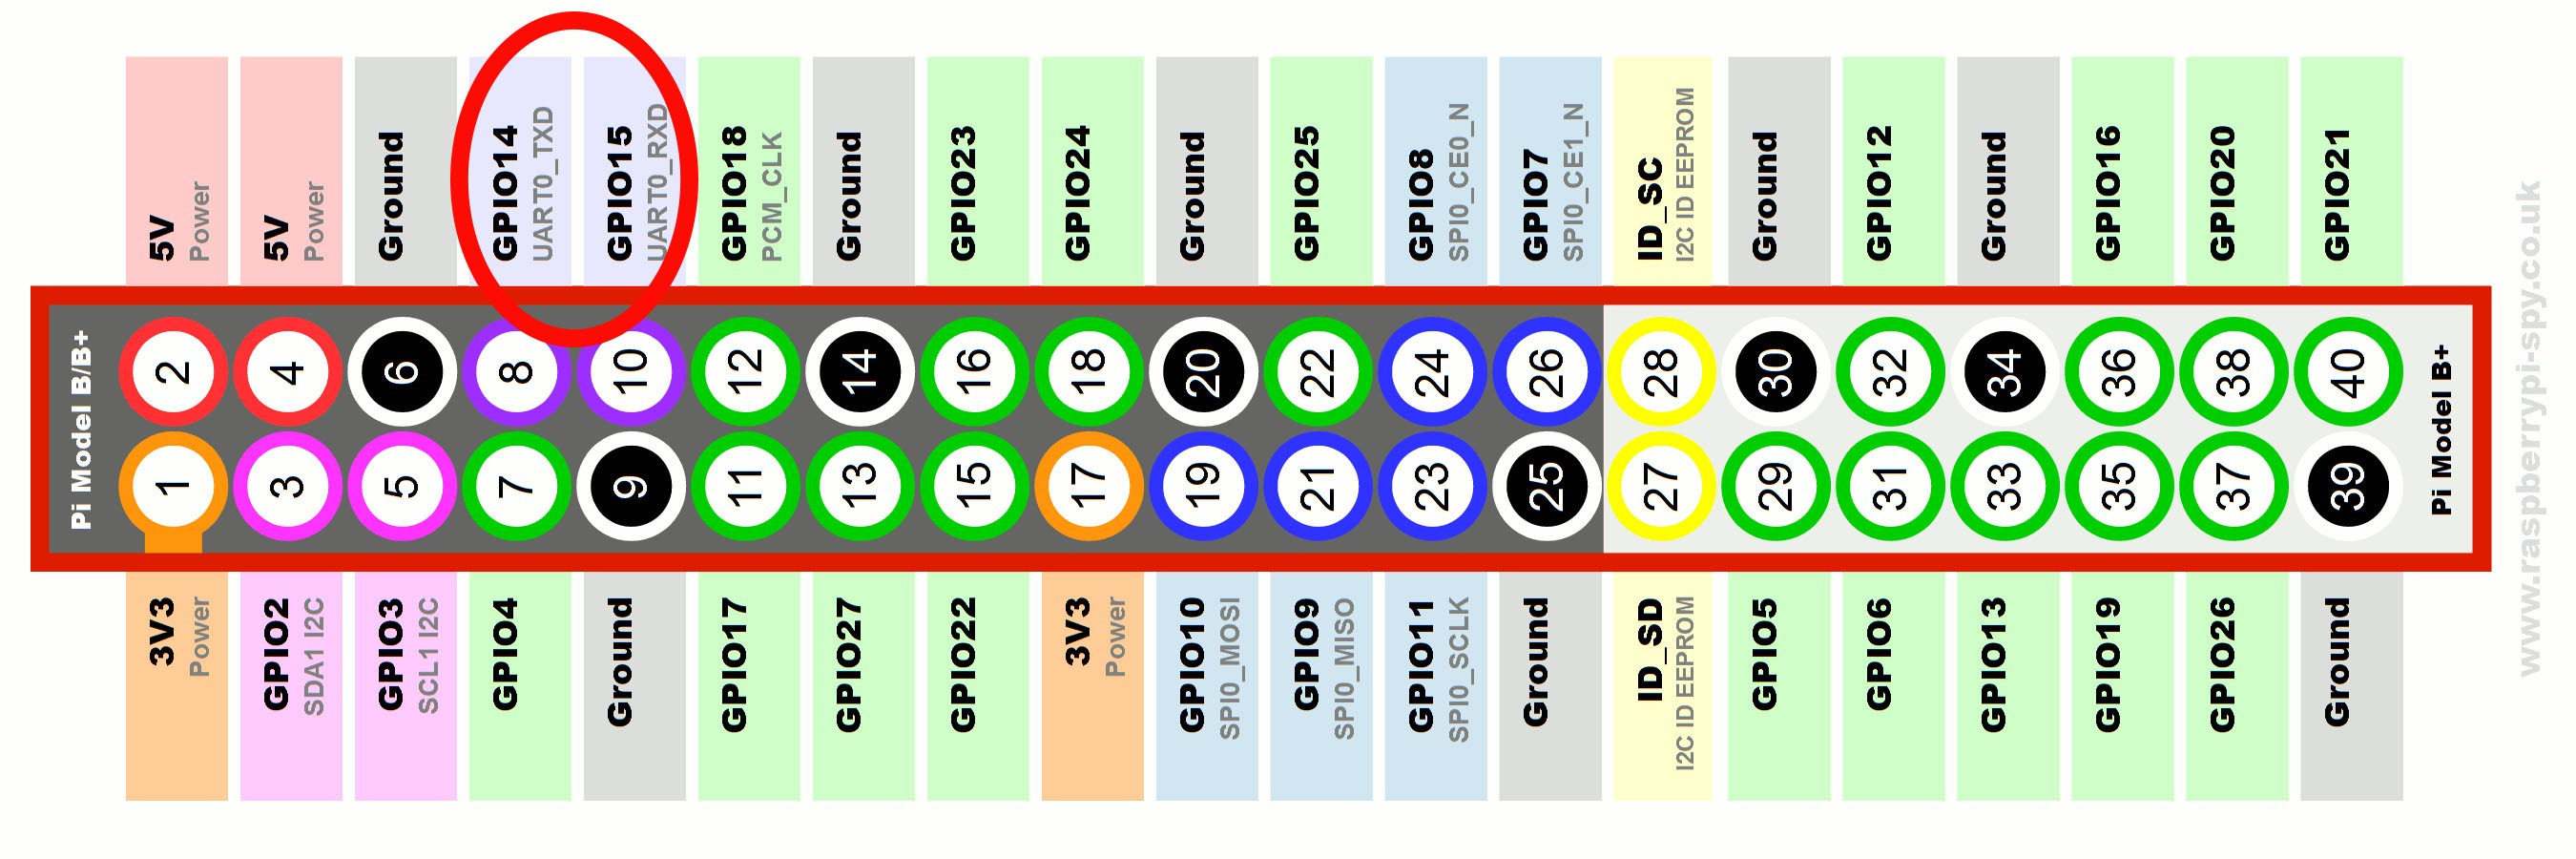
\includegraphics[scale=0.143]{tesi2.jpg}
 \caption[Figure 2]{Highlight of UART reserved GPIOs}\label{fig:seconda}
 \end{figure}

\subsubsection{UART0}
The UART0 is a fully fledged asynchronous serial interface, abiding to the 
PL011 ARM specification \cite{pl011}. To properly run on real hardware, the
corresponding pins must be configured to use the alternate function number 0 with
no internal pull up or down.
Its register are located starting at the address 0x3F201000, each of them
is 32 bits wide and they are organized as follows (some unimportant ones are omitted for brevity):
\begin{description}
    \item[Data:] this register contains the first character present in 
            the receive FIFO and can be written to send an outgoing character to 
            the transmit FIFO. Addidionally, it presents an error report of the ongoing
            connection, with a specific bit for every condition (overrun, break,
            parity, framing).
    \item[RSRECR:] a redundant register for error conditions.
    \item[Flag:] contains various flags on the current state of the UART, like 
            state (full or empty) of the transmit and receive FIFOs and whether
            the UART device is busy or idle.
    \item[IBRD:] integer part of the baudrate divisor: when configuring the device
            the baudrate is established as a floating point divisor prescaling
            the system clock. This is the integer part.
    \item[FBRD:] Floating point part of the baudrate divisor.
    \item[Line control:] this register manages configuration options like
            parity, number of stop bits, word length and FIFO abilitation.
    \item[Control:] this register controls the actual peripheral; mainly used
            for enabling and disabling the whole device.
    \item[IFLS:] interrupt FIFO level selection register. It is used to establish 
            at which percentage each FIFO (transmit or receive) triggers the
            corresponding interrupt. Possible values range from 1/8 to 7/8.
    \item[Interrupt mask:] allows to mask specific interrupts tied to the peripheral,
            such as those fired on reception and transmission of a character
    \item[Raw interrupt:] read only register updated with currently pending
            interrupts, regardless of the mask settings.
    \item[Masked interrupt:] same as the raw interrupt register but with the
            masked interrupt lines excluded.
    \item[Interrupt clear:] register to be written to clear pending interrupts.
\end{description}

Of all those registers, the only ones a student should really care about are
data, flag, interrupt mask, masked interrupt and interrupt clear. All the others 
are used for the initialization of the peripheral, which is handled by the 
hardware abstraction layer and should not be changed.

The serial interface is configured as 8 bit wide, no parity bit and with
a baudrate of 115200. The FIFOs are disabled for simplicity, so they act like 
a one character deep buffer.

\subsubsection{UART1 or Mini UART}
The UART1 is part of the group of auxiliary peripherals, together with two SPI
interfaces. In comparison with UART0 it has much more restricted functionality,
but still enough for a simple educational project. For example, it does not 
provide framing error detection or parity bit management, features that are either
disabled or ignored even in its more complete counterpart.
To properly run on real harware, the corresponding pins must be set to use the
alternate function number 5 with no internal pull up or down.
Its registers are located starting at the address 0x3F215040, each of them is 32 bits
wide and they are organized as follows (some unimportant ones are omitted for brevity):

\begin{description}
    \item[IO:] reading from this register yield the first character present in the
            receive FIFO, while writing it inserts the data into the write FIFO.
    \item[IIR:] register for enabling receive and transmit interrupts. If the first
            bit is set an interrupt line is asserted whenever the transmission FIFO
            is empty; if the second bit is set an interrupt line is asserted whenever
            the reception FIFO is not empty.
    \item[IER:] register holding information about which interrupt is pending (if any).
    \item[LCR:] controls whether the Mini UART works in 8 bit or 7 bit mode.
    \item[LSR:] line control status; used to determine if the device is ready to 
            accept new data or if there are received characters to be read.
    \item[CNTL:] control register to enable (in a separate fashion if so requested)
            the receive and trasmit lines.
    \item[BAUD:] 16 bit baudrate counter, to be set directly to the desired value.
\end{description}
Again, since the abstraction layer takes care of the initialization procedure
the user should really care about four registers: IO, IIR, IER and LSR.
The serial configuration is the same as the UART0.

\section{Interrupt Controller}
\label{gic}
The BCM2837 SoC has at least two devices acting as interrupt controllers. One of 
them is clearly defined in the peripheral datasheet \cite{bcm2835}, while the
other is not clearly named but hinted at thorugh register definition in a later 
revision \cite{rev3.4}. Those are here arbitrarily named Base Interrupt Controller (BIC)
and Generic Interrupt Controller (GIC).
These two interrupt controllers are cascaded, meaning that 64 interrupt lines are 
wired to the BIC which in turn compresses them into 2 interrupt lines for the GIC
controller; additionally, the GIC also receives some interrupt lines from mailboxes
and USB.

 \begin{figure}[h]
 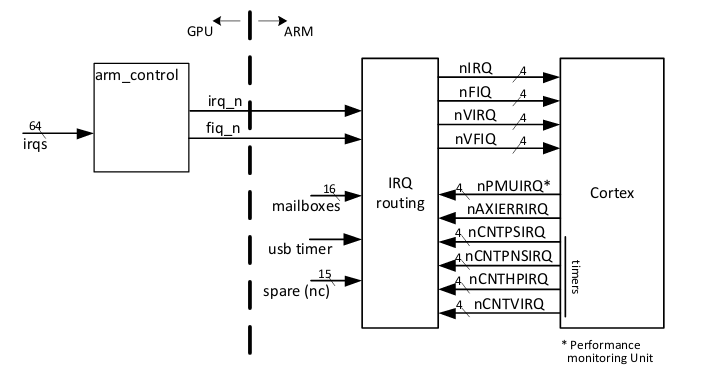
\includegraphics[scale=0.55]{tesi3.png}
 \caption[Figure 3]{BCM2837 interrupt controllers configuration}\label{fig:interrupt}
 \end{figure}
From a practical standpoint there are often serveral registers indicating which interrupt
line is being asserted at any moment. There is no apparent drawback in ignoring most
of them and just reading each device-specific register to discern which source fired
the exception.
The general interrupt organization is very confused and obscure. Interrupt functionality
was achieved mainly through examples and reverse engineering regarding the specific
device taken in consideration at the time.
What follows is a brief listing of interrupt related configuration for the devices
used in this work.

\begin{description}
    \item[UART] Both UART devices are cascated through the two interrupt controllers;
        although they can be checked via registers in both controllers, it is suggested
        to only read the Masked IRQ and IIR registers of the respective peripheral.
    \item[ARM timer] Being this an interrupt internal to the ARM processor its
        status has only been checked against the innermost interrupt controller (GIC).
        It is not clear whether it is present in the BIC as well.
    \item[Inter processor mailboxes] Possibly the sole source clearly
        depicted from the documentation, its presence can be understood from the 
        corresponding register in the Generic Interrupt Controller (as indicated
        by \ref{fig:interrupt}).
\end{description}

\subsection{Inter Processor Interrupt (IPI)}
In a multicore system such as the Raspberry Pi 3 the need arises for a privileged
communication channel between each core. The ARM Cortex-A53 does not provide an 
explicit method to do so, and it is left to the Generic Interrupt Controller to 
provide.
Similarly to the interface between ARM and Videocore there are mailboxes between
the four cores of the CPU as well.

The operation of those inter core mailboxes is much more straightforward than the
CPU-GPU counterpart. There are four for each core and for each mailbox the GIC
exposes three types control registers, for a total of 36 registers 
\footnote{Note: the first kind of register cover all four mailboxes for each core}.
\begin{description}
    \item[Mailbox Control] four registers of this type in total, one for each core
        and covering its four mailboxes. They enable an interrupt or fast interrupt
        line for each mailbox.
    \item[Mailbox Write-Set] four registers for each mailbox in every core, so 
        sixteen of them in total. They are write only and are used to put the
        actual data in the mailbox. Upon write the corresponding enabled exception
        (if any) is fired for the selected core.
    \item[Mailbox Read and Write-Clear] one register for each corresponding
        Write-Set register. They can be read to receive the data sent by writing
        in the Write-Set register, and have to be written to disarm the interrupt
        line. Each bit of the register is independent in firing the interrupt, so 
        to completely clear the same content that was read from the register must
        be written back on it.
\end{description}

\clearpage{\pagestyle{empty}\cleardoublepage}
\chapter{Emulated peripherals}
\label{emulated}
The Raspberry Pi 3 (or any other version or model) does not have many peripheral
devices to toy with. In part this is due to its heritage of low resource board, 
and in part to extensibility through four generic USB ports and 40-pin header,
allowing for a wide range of HAT (Hardware Attached on Top) extensions and external
USB devices.
In the perspective of an educational project however this is a severe limitation.
While $\mu$MPS2 and $\mu$ARM can each bring five device types with eight possible
instance per type, the Raspberry Pi has only two really usable devices: the 
two serial interfaces (that strongly resemble $\mu$MPS2 terminals).

Other options cannot be considered for multiple reasons:
\begin{itemize}
    \item The screen is simple and usable, but lacks educational value. It is 
        nothing more than a buffer to write on; the GPU then manages actually
        sending the data to the screen.
    \item The EMMC interface is far too complex to be used by students. The professor
        would need either to spend a great deal of time and effort to explain how
        it works or provide a library to access it, in contrast with the phylosophy
        of this work.
    \item The USB controller suffers a even worse degree of complexity, to the point
        that developing a support library would be a monumental task in itself.
        Last but not least, it is not supported by Qemu.
    \item The network interface is unfortunately not directly connected to the ARM
        but instead managed by the USB controller.
    \item Other auxiliary peripherals like the two SPI interfaces would be perfect
        for the task: although arguably too low level, many modern motherboards
        include SPI or I2C controlled peripherals, making it an intersting addition
        to the program. However, those are not supported by Qemu.
\end{itemize}

To mitigate this problem, three classes of new devices have been implemented as 
emulated peripherals in the hardware abstraction layer. Using $\mu$MPS2 as a reference,
these classes are tapes, disks and printers.

While building an entire emulator would give full control over the device interface,
in this work the emulation is carried on to the best level permitted by a bare
metal environment, leaking some imperfections on the exposed controls.

\section{Emulated Device Interface}
Initially emulated devices were made accessible via fake registers: simple pre-established
memory locations that were frequently polled by the abstraction layer.
Though most similar to the $\mu$MPS2 approach, this idea had significant flaws.
\begin{itemize}
    \item fake registers had no read or write limitations; location that should
        logically have been read only could be modified without limit, leaving
        the device in an incoherent state.
    \item polling was a frail mechanism, prone to error and race conditions. 
         A real device starts working the moment
        its registers are written, while in this scenario the user had to wait 
        for the contents to be read by the abstraction layer. This lead to 
        an unintuitive programming path, requiring the user to either poll 
        for changes in turn or use an {\tt swi} assembly instruction to wait for
        the polling interrupt.
    \item generally speaking, it is good practice to avoid polling when possible.
\end{itemize}

A solution was found that strays from the previous work's approach but better
fits the new environment and allows for a cleaner emulation: using mailboxes.

Some of the peripherals on the BCM2837 board are already managed by the GPU
through mailboxes, like the HDMI controller or the on-board activity led. In 
a very similar way, the abstraction layer is notified of a new command for printers,
tapes or disks by a write to the inter core communication mailbox.
Specifically, the mailbox 0 of the first core is reserved for emulated devices control.
This behaviour is transparent to the user because it raises a FIQ instead of a 
normal interrupt, and thus it can be received at any moment.

A command to a emulated device is then issued by writing some value to the mailbox
0 write-set register of the first core, found at memory address {\tt 0x40000080}.
The value must have the following format: the two least significant bits are the
device number and the two following bits are the device class.
The upper 28 most significant bits should point to a 16-byte aligned address containing
a register structure for the selected device.

\begin{figure}[h]
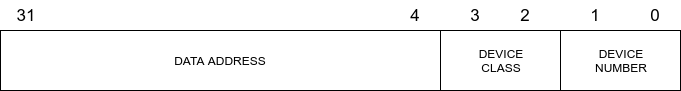
\includegraphics[scale=0.571]{tesi5.png}
\caption[Figure 5]{mailbox structure}\label{fig:mailbox}
\end{figure}

This should remind the reader of the mailbox communication protocol used by ARM
to talk with the Videocore, with the channel number encoded in the four least significant
bytes. Since it is a mechanism already present in the system it fits naturally
in the development process.

The ``register'' structure that should be pointer by the mailbox address is nearly 
identical to the device register layout in $\mu$MPS2 and $\mu$ARM.

\begin{table}[h]
\begin{center}
    \begin{tabular}{|c|c|c|c|}
    \hline
    \rowcolor[HTML]{C0C0C0} 
    Field \# & Address   & Field name & Size    \\ \hline
    0        & base+0x0  & STATUS     & 32 bits \\ \hline
    1        & base+0x4  & COMMAND    & 32 bits \\ \hline
    2        & base+0x8  & DATA0      & 32 bits \\ \hline
    3        & base+0xC  & DATA1      & 32 bits \\ \hline
    4        & base+0x10 & MAILBOX    & 32 bits \\ \hline
    \end{tabular}
 \caption[Table 1]{device register layout}\label{tab:reg}
\end{center}
\end{table}

Every device can have special functions for each register; what follows is a
general description.
\begin{description}
    \item[STATUS] contains the device state.
    \item[COMMAND] contains the command code to be executed.
    \item[DATA0 \& DATA1] carry additional arguments for the command.
    \item[MAILBOX] is written by the system to notify the command has been carried on.
\end{description}

Since this structure is nothing but a user memory location, fields like \textbf{STATUS}
and \textbf{MAILBOX} are uninitialized at first; only \textbf{COMMAND}, \textbf{DATA0} and \textbf{DATA1}
must contain proper data. Once the abstraction layer has received the fast interrupt
and parsed the registers it copies the internal state of the device onto the
provided memory location, populating all of its fields.

After receiving the mailbox the abstraction layer sets the \textbf{MAILBOX} field
to 1. This however does not mean the operation has been finished successfully, as 
real world devices take time to operate; as such, there are fabricated delays between
commands and execution.

Once the execution is complete an interrupt is asserted. Interrupt lines for emulated
devices are emulated as well with a memory location allocated for the task, at 
base address {\tt 0x0007F020}.

\begin{table}[h]
\begin{center}
    \begin{tabular}{|c|c|c|c|}
    \hline
    \rowcolor[HTML]{C0C0C0} 
    Interrupt line \# & Address  & Device class & Size   \\ \hline
    0                 & base+0x0 & Timer        & 8 bits \\ \hline
    1                 & base+0x1 & Disk         & 8 bits \\ \hline
    2                 & base+0x2 & Tape         & 8 bits \\ \hline
    3                 & base+0x3 & Printer      & 8 bits \\ \hline
    \end{tabular}
 \caption[Table 2]{emulated interrupt lines}\label{tab:reg}
\end{center}
\end{table}

\section{Tapes}
Four instance of the tape device are supported. They are read only and work as if 
queried through a DMA system.
The tape can be viewed as a sequential list of 4KiB blocks. each block is marked 
with a 4 bytes delimiter denoting the content of the underlying block.


\section{Disks}

\section{Printers}



\clearpage{\pagestyle{empty}\cleardoublepage}
\chapter{Project Internals}
In this chapter we describe in reasonable detail the source code of the 
project. The discussion will tipically hover at a structural level, depicting 
the design choices and code organization. This part will be most interesting for
those with the intent of maintaining of modifying the work, or to study ARM
bare metal development.

The size of the project is comparatively small, only reaching about 4000 lines of 
code. The real weight of this work does not lie in the actual software that was
written but in the idea and study of the environment, pioneering the possibility
of developing a proof-of-concept OS on real hardware instead of an emulator.

\section{Design Principles and Overall Structure}
Besides creating a convenient abstraction layer, the whole code base is written 
with the goal of being an understandable example of bare metal development. Particular 
care is taken in making sure that every function is readable and understandable
with a single glance even out of context and in using descriptive, self-explanatory
names. Where deemed necessary, comments help to further exaplain what is happening.

Source files can be grouped in three main categories. First, the core of the abstraction
layer is comprised basically of the assembler entry point, the C entry point and
the interrupt handling routines. Second, a small library used internally to 
access hardware peripherals; logging routines, microSD card reading and writing, 
timer management. Third are the modules of the emulated devices like tapes and
printers, leaning on the previous utilities to create the illusion of physical
peripherals.

\subsection{Implementation Language}
The choice of language is severely limited by the bare environment and fell unsurprisingly
on C and Assembly. Such basic programming languages contribute to the overall simplicity,
as there are no particular patterns or constructs used beside raw memory management.

The Assembler compoment was kept to a minimum for ease of understanding; from
the moment the C stack is available there is no real reason not to jump into 
C code (unless the goal was to exercise Assembly programming, which is not our case).

Thus, there are only two Assembly source files: {\tt init.S} is the absolute first
entry point and provides initialization for system registers, interrupt vectors, 
bss section and multicore functionality; {\tt asmlib.S} contains utility functions
that make heavy use of general and specific purpose registers that would have
required inline Assembly instructions anyway if implemented in C.

\subsection{Build Tools}
Contrarily to the $\mu$MPS family of emulators, this work does not use the 
Autotool suite of building tools (GNU Automake and Autoconf) to manage source 
compilation and package installation.
Not having a newly created graphical interface there are no library dependencies
such as Qt, weakening the need for strict dependency check. 
This, together with a smaller overall codebase prompted the author to search 
for a simpler and more modern build tool, and the final choice is Scons.

Scons has the advantage of being much more flexible and easy to use when compared
to older tools. Instead of leaning on a brand new (and potentially cumbersome)
language to configure the build process it relies on an already existing one, well
received and praised for its approachable syntax: Python.

In fact, Scons can be assimilated to a Python library for declaring build dependency
trees. Its philosophy is similar to make but brings a much cleaner syntax and 
user control over the process. 

\subsection{Linker Script}
The linker script is an essential piece when compiling for the Raspberry Pi 3. It has
to specify {\tt 0x80000} as the loading address for compatibility reasons with Qemu
and it ensures the initialization code is at the very beginning of the kernel image.
It also allocates some memory as stack to be used by the abstraction layer interrupt
routines.

\section{Initialization}
After loading all necessary components, the on-board GPU launches ARM execution at 
address {\tt 0x80000}. There, we can find the compiled code from the 
{\tt init.S} Assembly file.
The first operations are:
\begin{enumerate}
    \item Enabling access at \textbf{EL0} and \textbf{EL1} to the internal ARM 
        timer registers.
    \item Setting a separate stack for each core for internal interrupt handling.
    \item Enabling AArch64 execution state.
    \item Moving the execution level to \textbf{EL1} \footnote{The Rasbperry Pi 3
     starts in \textbf{EL2}, while Qemu initially runs at \textbf{EL3}}.
    \item Setting up interrupt handling routines.
    \item Preparing execution for all cores: while the first core jumps to C code,
        the remaining ones are parked in a waiting loop, ready to be fired.
    \item The bss section (uninitialized data) is zeroed and the first core jumps
        to the {\tt bios\_main} function.
\end{enumerate}

From there control is passed to C, with another series of initialization routines:
\begin{enumerate}
    \item The memory locations dedicated to device emulation and user interrupts
        are cleared.
    \item Every real device is initialized: GPIOs, UARTs, EMMC, display.
    \item Every emulated device is initialized, building on the real hardware.
    \item Cores 1, 2 and 3 are unlocked from their parked state and set to 
        run an infinite wait loop.
    \item The user provided {\tt main} is called.
\end{enumerate}

\section{Interrupt Management}
The core of the abstraction layer lies in the interrupt handling routines. We refer
to the handlers predefined in the abstraction layer as internal interrupt handlers;
 the students should define their own handlers, from now on referred to as user defined handlers.
There are 4 possible (and real) IRQ sources:
\begin{enumerate}
    \item ARM timer
    \item UART0
    \item UART1
    \item Mailboxes
\end{enumerate}
The {\tt main} function is assumed to never return; inside it the user should
prepare an appropriate time slice and then start executing the first process.
The time slice is set using the {\tt setTIMER()} function.
Note that {\tt setTIMER()} does not interacts with the ARM timer directly but 
through an internal queue of virtual timers.
 Once the time slice is over the internal interrupt handler is called. It is 
 responsible for operating emulated devices, but other than that immediatly
 passes control to the user defined interrupt handler.

 \begin{figure}[h]
    \begin{center}
 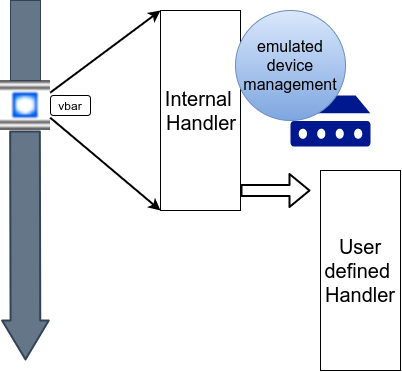
\includegraphics[scale=0.8]{tesi6.png}
 \caption[IRQ switch]{Interrupt handling schematic}\label{fig:irq}
    \end{center}
 \end{figure}

Other exception handlers, like the synchronous exception handler, are even 
simpler, reduced to passing control to the user defined routine if present.


\section{Emulated Devices}
The idea behind emulated peripherals and their fabricated interface 
have already beed described in Chapter \ref{emulated}. Here we give a more detailed 
presentation about the principle under which they work.

A command to an emulated device is issued through a mailbox. For coherency reasons
interrupts are however disabled at execution level \textbf{EL1} (the execution
level of user defined interrupts). To maintain this precaution and still allow 
user code running at \textbf{EL1} to be properly served when sending a command, the
special mailbox used for emulated peripherals fires a fast interrupt request (FIQ)
instead.
Fast interrupts are kept obscured to the user and managed only internally (in fact,
for this single purpose). IRQs and FIQs are separated for historical reasons, so 
the abstraction layer can disable the former and enable the latter.

Some commands require a two-step management to more closely resemble a real peripheral.
The first step is the fast interrupt, and is present for every command. For longer
operations a timer is set to be executed by a normal interrupt after a certain amount
of time.

\subsection{Timer Queue}
The second step of some device commands is scheduled for execution after a while;
since there is only one timer in the system to fire scheduled interrupts, this would
eventually overwrite other pending timers (namely the process time slice).
To prevent this internal timers uses a set of queue managing functions to 
schedule multiple timers at once. The ROM function {\tt setTIMER()} itself
just pushes a new timer onto the queue.

The queue is kept ordered from the first timer that will occur to the last.
When a interrupt is fired all the timers that were scheduled before the
current time are popped out of the queue, and the first remaining element (if any)
is scheduled again.

Interestingly, the implementation of this module is heavily inspired by the 
solution to phase 1 of the KayaOS project, covering process and semaphore queues.

\section{Hardware Library}
Modules under the {\tt source/hal/} subdirectory contain functions to conveniently access 
and use hardware peripherals. They serve a purpose mainly for usage internal to 
the project, as the abstraction layer does not normally expose those functions
(e.g. reading and writing the microSD card to emulate disk and tape devices).
They could however be seen as one of the many educational examples about 
bare metal programming for the BCM2837 and ARM processors in general.


\clearpage{\pagestyle{empty}\cleardoublepage}
\chapter{Student's Perspective}

\section{Memory Management Unit}

\clearpage{\pagestyle{empty}\cleardoublepage}
\chapter{Usage and Debugging}
\section{Final Result}
The final result of this work consists, from the user perspective, solely of 
two files: {\tt hal.elf} and {\tt hal.ld}.
The first is the the hardware abstraction layer compiled for an ARM64 target, 
containing system initialization and emulated devices management; the second is 
its linker script, to be used to link an application to the hal.

The hal performs all the necessary routines and then calls a {\tt main} function.
There is a weak-defined {\tt main} included with the hal that just echoes every
character received on UART0.
From there, the user provided code is expected to write specific memory addresses
to define new exception handlers and control emulated devices. 

One of the objectives of this work was to avoid creating ad hoc software and
relying as much as possible on widespread tools. Because of this, there is no
custom package like the $\mu$MPS2 emulator to install; instead the user needs
a proper cross compile toolchain for ARM64 (or an ARM64 device, like the Raspberry
Pi itself) and eventually Qemu.

Given a compiled elf with the user's code called {\tt app.elf} and assuming to
use {\tt aarch64-elf-gcc} as a cross compiler, the process to create a kernel image
would be 
\begin{lstlisting}
aarch64-elf-ld -nostdlib -nostartfiles -Thal.ld \
    -ooutput.elf hal.elf app.elf                                                                                                                                    
aarch64-elf-objcopy output.elf -O binary kernel8.img
\end{lstlisting}
The resulting binary can then be placed on a microSD card and run on a Raspberry Pi 3
or on Qemu

\section{Qemu}
Since version 2.12 Qemu supports a Raspberry Pi 3 emulated machine.
The official version for the Linux distro of choice may be less recent, in 
which case the user needs to compile the package from source.
 Particular care was taken in assuring the same code runs with no discernible difference on
the emulator and the device, which was not a difficult task.
Usually, in the rare situations where virtual and real boards differ in their
behaviour the real hardware is in the right (as one would expect).
Some examples found along the way are:
\begin{itemize}
    \item Uninitialized memory location will inevitably contain null values if 
        running under Qemu; the real world RAM is not so clement, and will live 
        up to the tale of having its content randomized after a reset.
    \item The MMU memory configuration includes distinguishing between device
        and normal memory: while the latter ban be subject to caching to increase performance,
        the former will not be optimized. Device memory is meant for memory mapped
        areas that are connected to peripherals, as their volatile nature would
        mix with caching for incoherent results.
        Failing to set the device area as device memory will be forgiven on Qemu
        as there are no real peripherals; instead, the Raspberry Pi board will most likely
        not behave as expected.
    \item Qemu is whimsical about the memory address where to load the kernel image.
        The emulator's boot sequence is different from the real device as the
        {\tt kernel8.img} file is not read from the microSD card but passed from
        the command line. Qemu invariably starts the execution by jumping at 
        {\tt 0x80000}; if that is not the same address referenced by the linker
        script the kernel will fail to run.
\end{itemize}

Qemu requires a kernel image and a microSD card image to be passed as command
line arguments. An example command to run the emulator is:
%TODO: specify how to create an image
\begin{lstlisting}
qemu-system-aarch64 -M raspi3 -kernel kernel8.img \
    -drive file=drive.dd,if=sd,format=raw \
    -serial vc -serial vc
\end{lstlisting}

Where the command line options have the following meaning:
\begin{description}
    \item[-M raspi3] specifies the machine to emulate.
    \item[-kernel kernel8.img] specifies the kernel image to run.
    \item[-drive file=drive.dd,if=sd,format=raw] attaches the microSD card, here
        using an image file. Note that a real device can be used in the same way,
        for example using {\tt file=/dev/mmcblk0}, allowing to run both on the
        board and the emulator with the same exact drive.
    \item[-serial vc] each serial option accounts for a UART interface (UART0 and UART1,
        in this order). {\tt vc} stands for ``virtual console'' and will open a 
        tab in the Qemu window. Another possible value is {\tt stdio}, which will
        conveniently pipe the serial output of the chosen interface on the shell
        (obviously available for only one of the two UARTs).
\end{description}

\section{Debugging}
The debug of the compiled kernel can be carried over Qemu with GDB. Using the
{\tt -gdb tcp:1234} parameter Qemu opens a debugging tcp port for a GDB client
to connect to (another port can be specified). The {\tt -s} command line flag 
brings the same result in a shorter format, and by adding {\tt -S} as well the
emulator will not start the execution, allowing the developer to connect.

Once the emulator is ready, a GDB client can connect to it. A client for
ARM64 should be present within the toolchain used to compile the kernel.
 A simple command line client may attach using the following commands (assuming
 the {\tt aarch64-elf-gcc} toolchain is installed)

\begin{lstlisting}
aarch64-elf-gdb
file output.elf
target remote localhost:1234
\end{lstlisting}

Emulators like $\mu$MPS2 have the prominent advantage of a specifically designed
running and debugging interface; nonetheless, a GDB server is a complete and
advanced debugging suite. The command line debugger may seem a scarce alternative,
but there are plenty of richer options; the author recommends {\tt gdbgui}, 
a browser-based Python GDB client.
Gdbgui can be installed via {\tt pip} or as an official package. It must be launched
with the {\tt --gdb} (or {\tt -g}) command line option to specify a proper GDB
client (i.e. the one found within the ARM64 toochain); it acts as a web server
reachable at the default port {\tt 5000} with any browser, and provides an intuitive
interface fitted with step-by-step debugging, memory inspection, threaded view and
so on.

 \begin{figure}[t]
 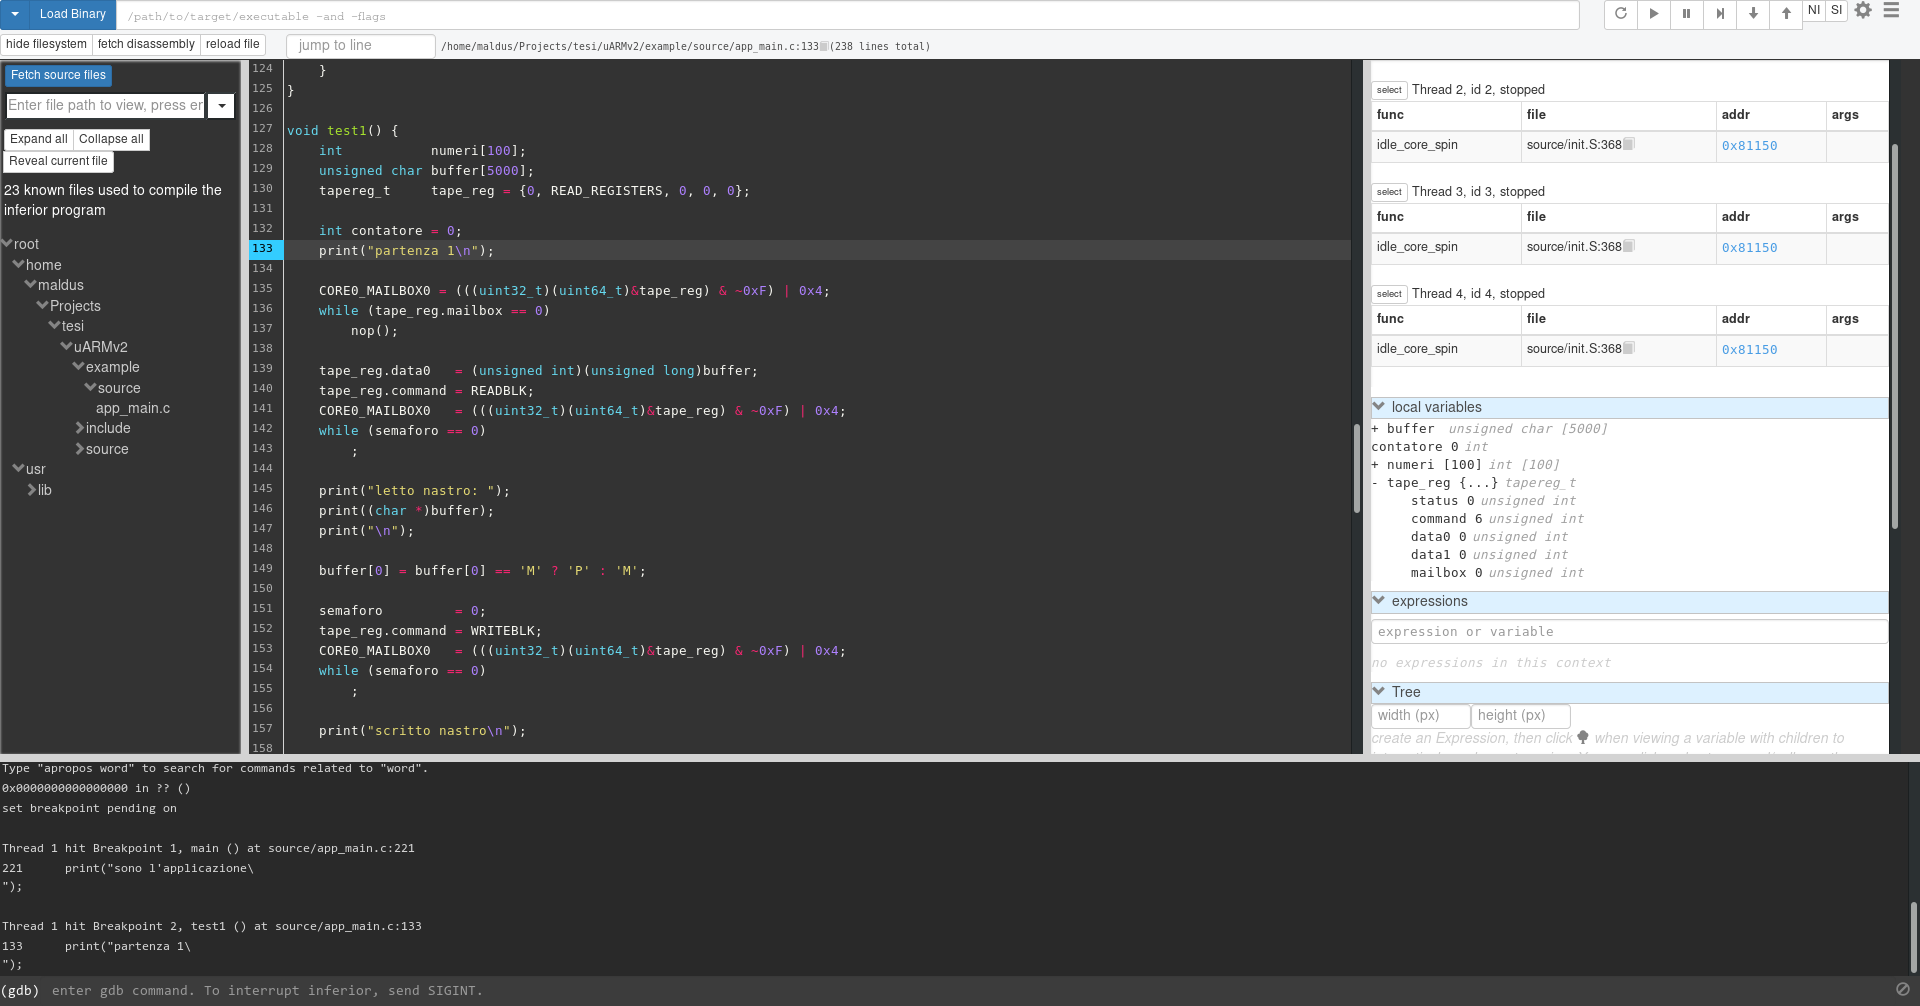
\includegraphics[scale=0.34,angle=-90,origin=c]{tesi4.png}
 \caption[Figure 4]{gdbgui browser interface}\label{fig:gdbgui}
 \end{figure}





%%%%%%%%%%%%%%%%%%%%%%%%%%%%%%%%%%%%%%%%%non numera l'ultima pagina sinistra
\clearpage{\pagestyle{empty}\cleardoublepage}
%%%%%%%%%%%%%%%%%%%%%%%%%%%%%%%%%%%%%%%%%per fare le conclusioni
\chapter{Conclusions and Future Work}
\section{Extending Qemu}
The recently added Raspberry Pi machine configuration for Qemu only supports a few
capabilities of the original board: the two serial interfaces, the framebuffer
display and the microSD card EMMC.
The biggest missing part is of course the USB controller (bringing around the
Network interface as well); the base complexity of the USB protocol, however,
 would probably make it an unsuitable choice for learning projects anyway.

Peripherals of less practical value in an emulator would perhaps end up being
most interesting in the scope of OS study. SPI and I2C are relatively
easy low level serial protocols that could make an interesting addition to the
learning program; same goes for the PCM audio interface and the whole GPIO 
header in general.
Qemu is a fairly flexible emulator, and a future improvement could focus on 
enriching the virtual environment with more device options.

\section{Debugging with GDB}
Being a off-the-shelf software GDB is flexible enough to be extended with 
a specifically tailored client. GDB provides a machine interpreter that recognizes
machine readable commands for the purpose of creating higher level interfaces.

If the generic approach of gdbgui was deemed too complex for inexperienced graduate
students one could implement a $\mu$MPS2-like debugging interface that connects
to the Qemu GDB server. Using the same interface but on a different note a
debugging environment could be created inside a commonly used IDE, like Atom or 
Visual Studio Code.

\section{Other ARM64 SoC}
Although it is now firmly seated in the Olympus of open source educational boards,
the Raspberry Pi family is build on awfully obscured and undocumented hardware.
Broadcom follows the market trend of not releasing any information on its 
products like other manufacturers.
There are many Raspberry Pi-like boards that base themselves on similar hardware:
namely, a potent ARM CPU assisted by a graphical processing unit. In principle,
the work that has been done for the British board could be easily ported to a 
wide number of similar devices. The Pine64 family, for example, has recently
marketed a laptop powered by one of their compute modules. Running a toy
OS on a real laptop could be a even higher highlight for an undergraduate
or even graduate student.

\begin{thebibliography}{90}             %crea l'ambiente bibliografia
\addcontentsline{toc}{chapter}{Bibliography}
%%%%%%%%%%%%%%%%%%%%%%%%%%%%%%%%%%%%%%%%%provare anche questo comando:
%%%%%%%%%%%\addcontentsline{toc}{chapter}{\numberline{}{Bibliografia}}
\bibitem{minix} Andrew S. Woodhull, Andrew S. Tanenbaum, 
                Operating System Design and Implementation, 1997.
\bibitem{bakingpi} University of Cambridge, Department of Computer Science and Technology,
                    Baking Pi - Operating Systems Development,
                    \url{https://www.cl.cam.ac.uk/projects/raspberrypi/tutorials/os/}
\bibitem{davolimorsiani} M. Goldweber, R. Davoli, and M. Morsiani,
                        \"The Kaya OS project and the $\mu$MPS hardware emulator\",
                          SIGCSE Bull., vol. 37, pp. 49-53, June 2005.
\bibitem{tesijonjic} T. Jonjic,
                    \"Design and Implementation of the $\mu$MPS2 Educational Emulator\",
                    Alma Mater Studiorum, 2012.
\bibitem{tesimelletti} M. Melletti,
                    \"Studio e Realizzazione dell'emulatore $\mu$ARM e del progetto
                    JaeOS per la Didattica dei Sistemi Operativi\",
                    Alma Mater Studiorum, 2016.
\bibitem{pop} M. Goldweber, R. Davoli, $\mu$MPS Principles of Operation, Lulu Books, 2011
\bibitem{ultibo} The Ultibo Project, \url{https://ultibo.org/}
\bibitem{circle} The Circle C++ environment, \url{https://github.com/rsta2/circle}
\bibitem{bcm2835} BCM2835 ARM Peripherals, Broadcom.
\bibitem{rev3.4} ARM Quad A7 Core, Broadcom.
\bibitem{pl011} PrimeCell UART (PL011) Technical Reference Manual, ARM.
\bibitem{guide} ARM Cortex-A Series Programmer's Guide for ARMv8-A, ARM, 2015.
\bibitem{armarm} ARM Architectural Reference Manual ARMv8, for ARMv8-A Architecture Profile, ARM, 2017.
\end{thebibliography}
%%%%%%%%%%%%%%%%%%%%%%%%%%%%%%%%%%%%%%%%%non numera l'ultima pagina sinistra
\clearpage{\pagestyle{empty}\cleardoublepage}
\chapter*{Ringraziamenti}
\thispagestyle{empty}
Qui possiamo ringraziare il mondo intero!!!!!!!!!!\\
Ovviamente solo se uno vuole, non \`e obbligatorio.
\end{document}
